\documentclass[twoside]{book}

% Packages required by doxygen
\usepackage{calc}
\usepackage{doxygen}
\usepackage{graphicx}
\usepackage[utf8]{inputenc}
\usepackage{makeidx}
\usepackage{multicol}
\usepackage{multirow}
\usepackage{textcomp}
\usepackage[table]{xcolor}

% Font selection
\usepackage[T1]{fontenc}
\usepackage{mathptmx}
\usepackage[scaled=.90]{helvet}
\usepackage{courier}
\usepackage{amssymb}
\usepackage{sectsty}
\renewcommand{\familydefault}{\sfdefault}
\allsectionsfont{%
  \fontseries{bc}\selectfont%
  \color{darkgray}%
}
\renewcommand{\DoxyLabelFont}{%
  \fontseries{bc}\selectfont%
  \color{darkgray}%
}

% Page & text layout
\usepackage{geometry}
\geometry{%
  a4paper,%
  top=2.5cm,%
  bottom=2.5cm,%
  left=2.5cm,%
  right=2.5cm%
}
\tolerance=750
\hfuzz=15pt
\hbadness=750
\setlength{\emergencystretch}{15pt}
\setlength{\parindent}{0cm}
\setlength{\parskip}{0.2cm}
\makeatletter
\renewcommand{\paragraph}{%
  \@startsection{paragraph}{4}{0ex}{-1.0ex}{1.0ex}{%
    \normalfont\normalsize\bfseries\SS@parafont%
  }%
}
\renewcommand{\subparagraph}{%
  \@startsection{subparagraph}{5}{0ex}{-1.0ex}{1.0ex}{%
    \normalfont\normalsize\bfseries\SS@subparafont%
  }%
}
\makeatother

% Headers & footers
\usepackage{fancyhdr}
\pagestyle{fancyplain}
\fancyhead[LE]{\fancyplain{}{\bfseries\thepage}}
\fancyhead[CE]{\fancyplain{}{}}
\fancyhead[RE]{\fancyplain{}{\bfseries\leftmark}}
\fancyhead[LO]{\fancyplain{}{\bfseries\rightmark}}
\fancyhead[CO]{\fancyplain{}{}}
\fancyhead[RO]{\fancyplain{}{\bfseries\thepage}}
\fancyfoot[LE]{\fancyplain{}{}}
\fancyfoot[CE]{\fancyplain{}{}}
\fancyfoot[RE]{\fancyplain{}{\bfseries\scriptsize Generated on Sat Feb 25 2017 16\-:52\-:03 for My Project by Doxygen }}
\fancyfoot[LO]{\fancyplain{}{\bfseries\scriptsize Generated on Sat Feb 25 2017 16\-:52\-:03 for My Project by Doxygen }}
\fancyfoot[CO]{\fancyplain{}{}}
\fancyfoot[RO]{\fancyplain{}{}}
\renewcommand{\footrulewidth}{0.4pt}
\renewcommand{\chaptermark}[1]{%
  \markboth{#1}{}%
}
\renewcommand{\sectionmark}[1]{%
  \markright{\thesection\ #1}%
}

% Indices & bibliography
\usepackage{natbib}
\usepackage[titles]{tocloft}
\setcounter{tocdepth}{3}
\setcounter{secnumdepth}{5}
\makeindex

% Hyperlinks (required, but should be loaded last)
\usepackage{ifpdf}
\ifpdf
  \usepackage[pdftex,pagebackref=true]{hyperref}
\else
  \usepackage[ps2pdf,pagebackref=true]{hyperref}
\fi
\hypersetup{%
  colorlinks=true,%
  linkcolor=blue,%
  citecolor=blue,%
  unicode%
}

% Custom commands
\newcommand{\clearemptydoublepage}{%
  \newpage{\pagestyle{empty}\cleardoublepage}%
}


%===== C O N T E N T S =====

\begin{document}

% Titlepage & ToC
\hypersetup{pageanchor=false}
\pagenumbering{roman}
\begin{titlepage}
\vspace*{7cm}
\begin{center}%
{\Large My Project }\\
\vspace*{1cm}
{\large Generated by Doxygen 1.8.5}\\
\vspace*{0.5cm}
{\small Sat Feb 25 2017 16:52:03}\\
\end{center}
\end{titlepage}
\clearemptydoublepage
\tableofcontents
\clearemptydoublepage
\pagenumbering{arabic}
\hypersetup{pageanchor=true}

%--- Begin generated contents ---
\chapter{Program 1 -\/ S\-D\-S\-M\&T Paint}
\label{index}\hypertarget{index}{}\hypertarget{index_course_section}{}\section{Course Information}\label{index_course_section}
\begin{DoxyAuthor}{Authors}
Luke Videckis and Jeffrey Ross
\end{DoxyAuthor}
\begin{DoxyDate}{Date}
February 24, 2017
\end{DoxyDate}
\begin{DoxyParagraph}{Instructor\-:}
Dr. Hinker
\end{DoxyParagraph}
\begin{DoxyParagraph}{Course\-:}
C\-S\-C 300 -\/ Section 1 -\/ 10\-:00 am
\end{DoxyParagraph}
\begin{DoxyParagraph}{Location\-:}
Mc\-Laury -\/ Room 205
\end{DoxyParagraph}
\begin{DoxyParagraph}{Description\-:}
This program immitates Microsoft Paint with less features. There is a palette in the bottom left corner of the window. Shapes can be selected by left clicking. Border colors are chosen by left clicking and fill colors are chosen by right clicking. The top left square of the palette shows the current color. Shapes are drawn by left clicking and dragging in the canvas. Shapes which are drawn can be moved by right clicking and dragging. When a shape is moved, it is redrawn on top of all other shapes.\par
\par
 This project is an exercise in O\-O\-P, G\-U\-I developement in Glut, practicing good repository citizenship, and working in a team.
\end{DoxyParagraph}
\hypertarget{index_compile_section}{}\section{Compiling and Usage}\label{index_compile_section}
\begin{DoxyParagraph}{Compiling Instructions\-:}
\% make to compile, \% ./main to run
\end{DoxyParagraph}
\begin{DoxyParagraph}{Usage\-:}
\begin{DoxyVerb}  c:\> main.exe
  d:\> C:\Project1\end{DoxyVerb}

\end{DoxyParagraph}
\hypertarget{index_todo_bugs_modification_section}{}\section{Todo, Bugs, and Modifications}\label{index_todo_bugs_modification_section}
\begin{DoxyRefDesc}{Bug}
\item[\hyperlink{bug__bug000001}{Bug}]None\end{DoxyRefDesc}


\begin{DoxyRefDesc}{Todo}
\item[\hyperlink{todo__todo000001}{Todo}]None\end{DoxyRefDesc}


\begin{DoxyParagraph}{Modifications and Development Timeline\-:}
\begin{DoxyVerb}Date          Modification
------------  --------------------------------------------------------------
https://gitlab.mcs.sdsmt.edu/7275982/Project1.git
\end{DoxyVerb}
 
\end{DoxyParagraph}

\chapter{Todo List}
\label{todo}
\hypertarget{todo}{}

\begin{DoxyRefList}
\item[\label{todo__todo000001}%
\hypertarget{todo__todo000001}{}%
page \hyperlink{index}{Program 1 -\/ S\-D\-S\-M\&T Paint} ]None
\end{DoxyRefList}
\chapter{Bug List}
\label{bug}
\hypertarget{bug}{}

\begin{DoxyRefList}
\item[\label{bug__bug000001}%
\hypertarget{bug__bug000001}{}%
page \hyperlink{index}{Program 1 -\/ S\-D\-S\-M\&T Paint} ]None
\end{DoxyRefList}
\chapter{Hierarchical Index}
\section{Class Hierarchy}
This inheritance list is sorted roughly, but not completely, alphabetically\-:\begin{DoxyCompactList}
\item \contentsline{section}{current\-Properties}{\pageref{structcurrentProperties}}{}
\item \contentsline{section}{Shape}{\pageref{classShape}}{}
\begin{DoxyCompactList}
\item \contentsline{section}{Ellipse}{\pageref{classEllipse}}{}
\begin{DoxyCompactList}
\item \contentsline{section}{Filled\-Ellipse}{\pageref{classFilledEllipse}}{}
\end{DoxyCompactList}
\item \contentsline{section}{Line}{\pageref{classLine}}{}
\item \contentsline{section}{Rectangle}{\pageref{classRectangle}}{}
\begin{DoxyCompactList}
\item \contentsline{section}{Filled\-Rectangle}{\pageref{classFilledRectangle}}{}
\end{DoxyCompactList}
\end{DoxyCompactList}
\end{DoxyCompactList}

\chapter{Class Index}
\section{Class List}
Here are the classes, structs, unions and interfaces with brief descriptions\-:\begin{DoxyCompactList}
\item\contentsline{section}{\hyperlink{structcurrentProperties}{current\-Properties} \\*This is the \hyperlink{classShape}{Shape} class }{\pageref{structcurrentProperties}}{}
\item\contentsline{section}{\hyperlink{classEllipse}{Ellipse} \\*This is the \hyperlink{classEllipse}{Ellipse} Class. It inherits from the \hyperlink{classShape}{Shape} class }{\pageref{classEllipse}}{}
\item\contentsline{section}{\hyperlink{classFilledEllipse}{Filled\-Ellipse} \\*This is the \hyperlink{classFilledEllipse}{Filled\-Ellipse} Class. It inherits from the \hyperlink{classEllipse}{Ellipse} class }{\pageref{classFilledEllipse}}{}
\item\contentsline{section}{\hyperlink{classFilledRectangle}{Filled\-Rectangle} \\*This is the \hyperlink{classFilledRectangle}{Filled\-Rectangle} Class. It inherits from the \hyperlink{classRectangle}{Rectangle} class }{\pageref{classFilledRectangle}}{}
\item\contentsline{section}{\hyperlink{classLine}{Line} \\*This is the \hyperlink{classLine}{Line} class. It inherits from the \hyperlink{classShape}{Shape} class }{\pageref{classLine}}{}
\item\contentsline{section}{\hyperlink{classRectangle}{Rectangle} \\*This is the \hyperlink{classRectangle}{Rectangle} Class. It inherits from the \hyperlink{classShape}{Shape} class }{\pageref{classRectangle}}{}
\item\contentsline{section}{\hyperlink{classShape}{Shape} \\*This is the \hyperlink{classShape}{Shape} class }{\pageref{classShape}}{}
\end{DoxyCompactList}

\chapter{File Index}
\section{File List}
Here is a list of all documented files with brief descriptions\-:\begin{DoxyCompactList}
\item\contentsline{section}{\hyperlink{ellipse_8cpp}{ellipse.\-cpp} }{\pageref{ellipse_8cpp}}{}
\item\contentsline{section}{\hyperlink{ellipse_8h}{ellipse.\-h} }{\pageref{ellipse_8h}}{}
\item\contentsline{section}{\hyperlink{FilledEllipse_8cpp}{Filled\-Ellipse.\-cpp} }{\pageref{FilledEllipse_8cpp}}{}
\item\contentsline{section}{\hyperlink{FilledEllipse_8h}{Filled\-Ellipse.\-h} }{\pageref{FilledEllipse_8h}}{}
\item\contentsline{section}{\hyperlink{FilledRectangle_8cpp}{Filled\-Rectangle.\-cpp} }{\pageref{FilledRectangle_8cpp}}{}
\item\contentsline{section}{\hyperlink{FilledRectangle_8h}{Filled\-Rectangle.\-h} }{\pageref{FilledRectangle_8h}}{}
\item\contentsline{section}{\hyperlink{functions_8cpp}{functions.\-cpp} }{\pageref{functions_8cpp}}{}
\item\contentsline{section}{\hyperlink{functions_8h}{functions.\-h} }{\pageref{functions_8h}}{}
\item\contentsline{section}{\hyperlink{line_8cpp}{line.\-cpp} }{\pageref{line_8cpp}}{}
\item\contentsline{section}{\hyperlink{line_8h}{line.\-h} }{\pageref{line_8h}}{}
\item\contentsline{section}{\hyperlink{rectangle_8cpp}{rectangle.\-cpp} }{\pageref{rectangle_8cpp}}{}
\item\contentsline{section}{\hyperlink{rectangle_8h}{rectangle.\-h} }{\pageref{rectangle_8h}}{}
\item\contentsline{section}{\hyperlink{shape_8h}{shape.\-h} }{\pageref{shape_8h}}{}
\end{DoxyCompactList}

\chapter{Class Documentation}
\hypertarget{structcurrentProperties}{\section{current\-Properties Struct Reference}
\label{structcurrentProperties}\index{current\-Properties@{current\-Properties}}
}


This is the \hyperlink{classShape}{Shape} class.  




{\ttfamily \#include $<$shape.\-h$>$}

\subsection*{Public Attributes}
\begin{DoxyCompactItemize}
\item 
float \hyperlink{structcurrentProperties_a444727aa40fea7fd0020434b7ebc9245}{color} \mbox{[}3\mbox{]}
\item 
float \hyperlink{structcurrentProperties_aa67742be2101d7049d5503f7d5a2e3a5}{border} \mbox{[}3\mbox{]}
\item 
int \hyperlink{structcurrentProperties_a3fb7d1d3f56132c1530f1a2a307a3172}{shape\-Type}
\item 
bool \hyperlink{structcurrentProperties_a73bc7474c39c0b1580577ad635074c67}{ready}
\end{DoxyCompactItemize}


\subsection{Detailed Description}
This is the \hyperlink{classShape}{Shape} class. 

\subsection{Member Data Documentation}
\hypertarget{structcurrentProperties_aa67742be2101d7049d5503f7d5a2e3a5}{\index{current\-Properties@{current\-Properties}!border@{border}}
\index{border@{border}!currentProperties@{current\-Properties}}
\subsubsection[{border}]{\setlength{\rightskip}{0pt plus 5cm}float current\-Properties\-::border\mbox{[}3\mbox{]}}}\label{structcurrentProperties_aa67742be2101d7049d5503f7d5a2e3a5}
R\-G\-B colors for the border \hypertarget{structcurrentProperties_a444727aa40fea7fd0020434b7ebc9245}{\index{current\-Properties@{current\-Properties}!color@{color}}
\index{color@{color}!currentProperties@{current\-Properties}}
\subsubsection[{color}]{\setlength{\rightskip}{0pt plus 5cm}float current\-Properties\-::color\mbox{[}3\mbox{]}}}\label{structcurrentProperties_a444727aa40fea7fd0020434b7ebc9245}
R\-G\-B colors for the fill color \hypertarget{structcurrentProperties_a73bc7474c39c0b1580577ad635074c67}{\index{current\-Properties@{current\-Properties}!ready@{ready}}
\index{ready@{ready}!currentProperties@{current\-Properties}}
\subsubsection[{ready}]{\setlength{\rightskip}{0pt plus 5cm}bool current\-Properties\-::ready}}\label{structcurrentProperties_a73bc7474c39c0b1580577ad635074c67}
set to true if both color and shape are selected \hypertarget{structcurrentProperties_a3fb7d1d3f56132c1530f1a2a307a3172}{\index{current\-Properties@{current\-Properties}!shape\-Type@{shape\-Type}}
\index{shape\-Type@{shape\-Type}!currentProperties@{current\-Properties}}
\subsubsection[{shape\-Type}]{\setlength{\rightskip}{0pt plus 5cm}int current\-Properties\-::shape\-Type}}\label{structcurrentProperties_a3fb7d1d3f56132c1530f1a2a307a3172}
1 = rectangle, 2 = ellipse, 3 = line, 4 = filled elipse, 5 = filled rectangle 

The documentation for this struct was generated from the following file\-:\begin{DoxyCompactItemize}
\item 
\hyperlink{shape_8h}{shape.\-h}\end{DoxyCompactItemize}

\hypertarget{classEllipse}{\section{Ellipse Class Reference}
\label{classEllipse}\index{Ellipse@{Ellipse}}
}


This is the \hyperlink{classEllipse}{Ellipse} Class. It inherits from the \hyperlink{classShape}{Shape} class.  




{\ttfamily \#include $<$ellipse.\-h$>$}

Inheritance diagram for Ellipse\-:\begin{figure}[H]
\begin{center}
\leavevmode
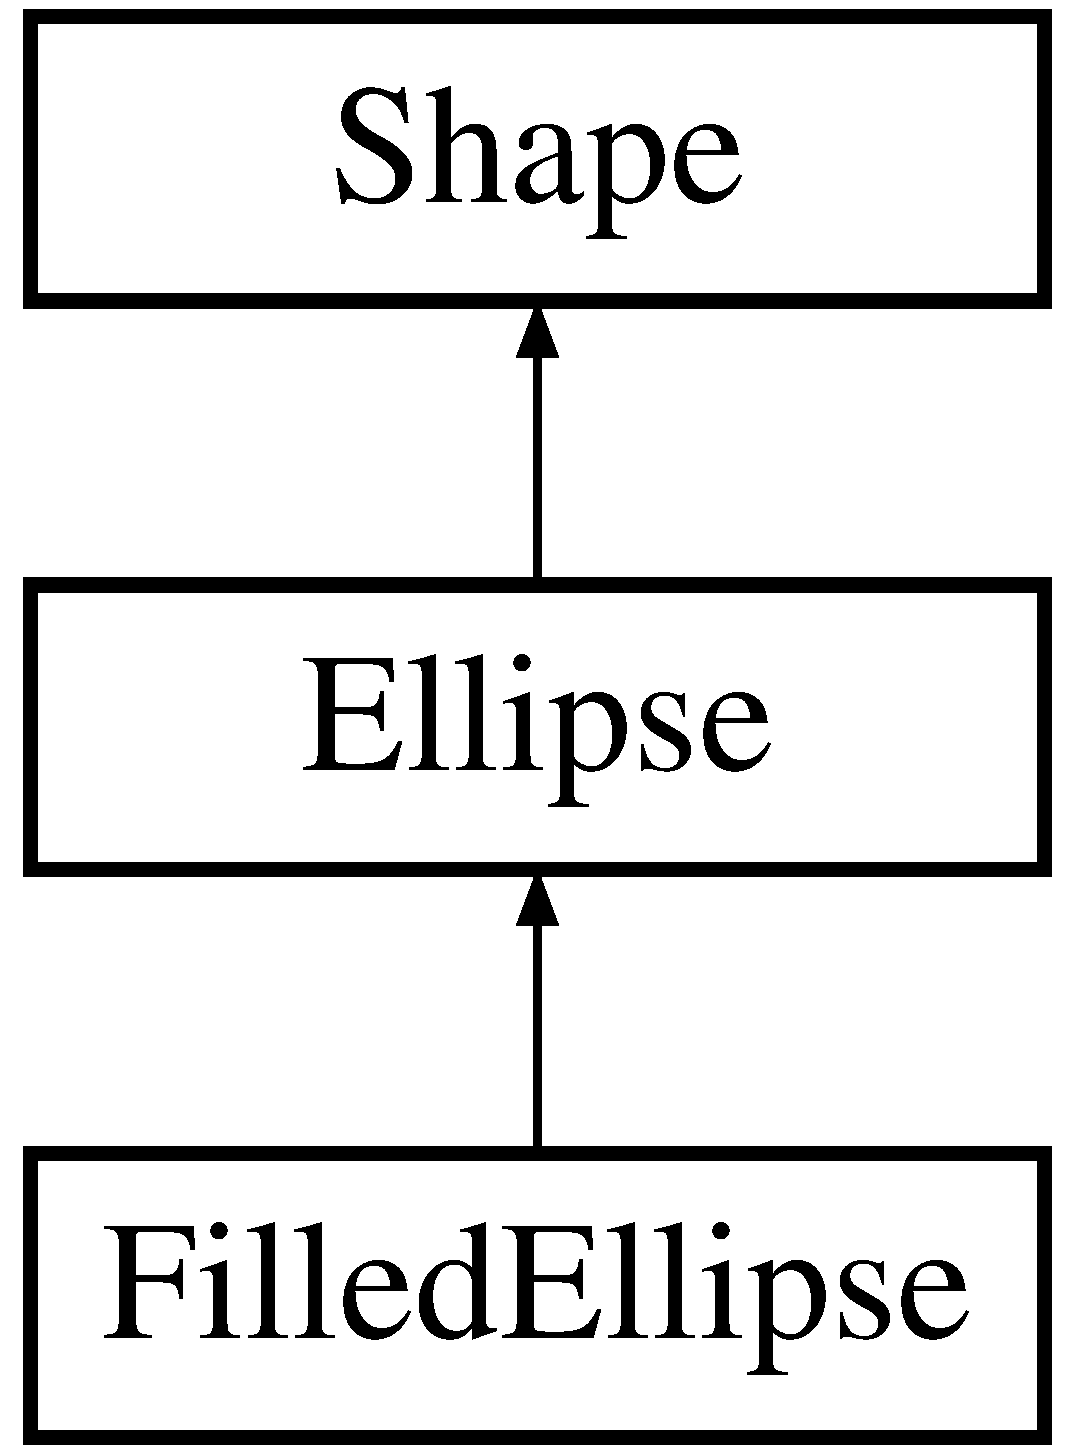
\includegraphics[height=3.000000cm]{classEllipse}
\end{center}
\end{figure}
\subsection*{Public Member Functions}
\begin{DoxyCompactItemize}
\item 
\hyperlink{classEllipse_a03fdd8cc5f0d18626a2679ac4a733485}{Ellipse} (int in\-X1, int in\-Y1, int in\-X2, int in\-Y2, float in\-Color\mbox{[}3\mbox{]})
\item 
\hyperlink{classEllipse_a94271a8a2b16101a52491b7e81e28547}{$\sim$\-Ellipse} ()
\item 
void \hyperlink{classEllipse_a99c72122041b0523dc9227fc3e985179}{draw} () const 
\item 
bool \hyperlink{classEllipse_a31b6310abda060741eb7033636709ce6}{contains} (int a, int b) const 
\item 
void \hyperlink{classEllipse_a7b536dcba1a231980299d2f309ab6fe0}{move} (int x, int y)
\end{DoxyCompactItemize}
\subsection*{Additional Inherited Members}


\subsection{Detailed Description}
This is the \hyperlink{classEllipse}{Ellipse} Class. It inherits from the \hyperlink{classShape}{Shape} class. 

\subsection{Constructor \& Destructor Documentation}
\hypertarget{classEllipse_a03fdd8cc5f0d18626a2679ac4a733485}{\index{Ellipse@{Ellipse}!Ellipse@{Ellipse}}
\index{Ellipse@{Ellipse}!Ellipse@{Ellipse}}
\subsubsection[{Ellipse}]{\setlength{\rightskip}{0pt plus 5cm}Ellipse\-::\-Ellipse (
\begin{DoxyParamCaption}
\item[{int}]{in\-X1, }
\item[{int}]{in\-Y1, }
\item[{int}]{in\-X2, }
\item[{int}]{in\-Y2, }
\item[{float}]{in\-Color\mbox{[}3\mbox{]}}
\end{DoxyParamCaption}
)}}\label{classEllipse_a03fdd8cc5f0d18626a2679ac4a733485}
ellipse constructor

\begin{DoxyAuthor}{Author}
Luke Videckis
\end{DoxyAuthor}
\begin{DoxyParagraph}{Description\-:}
This is the constructor for the \hyperlink{classEllipse}{Ellipse} class. It just updates the values for the class. (no way!)
\end{DoxyParagraph}

\begin{DoxyParams}[1]{Parameters}
\mbox{\tt in}  & {\em in\-X1} & -\/ the x value of the down click \\
\hline
\mbox{\tt in}  & {\em in\-Y1} & -\/ the y value of the down click \\
\hline
\mbox{\tt in}  & {\em in\-X2} & -\/ the x value of the up click \\
\hline
\mbox{\tt in}  & {\em in\-Y2} & -\/ the y value of the up click \\
\hline
\mbox{\tt in}  & {\em in\-Color} & -\/ the float of R\-G\-B values for the \hyperlink{classEllipse}{Ellipse}\\
\hline
\end{DoxyParams}
\begin{DoxyReturn}{Returns}
nothing 
\end{DoxyReturn}
\hypertarget{classEllipse_a94271a8a2b16101a52491b7e81e28547}{\index{Ellipse@{Ellipse}!$\sim$\-Ellipse@{$\sim$\-Ellipse}}
\index{$\sim$\-Ellipse@{$\sim$\-Ellipse}!Ellipse@{Ellipse}}
\subsubsection[{$\sim$\-Ellipse}]{\setlength{\rightskip}{0pt plus 5cm}Ellipse\-::$\sim$\-Ellipse (
\begin{DoxyParamCaption}
{}
\end{DoxyParamCaption}
)}}\label{classEllipse_a94271a8a2b16101a52491b7e81e28547}
ellipse destructor

\begin{DoxyAuthor}{Author}
Luke Videckis
\end{DoxyAuthor}
\begin{DoxyParagraph}{Description\-:}
This is the destructor for the \hyperlink{classEllipse}{Ellipse} class. It also does absolutely nothing.
\end{DoxyParagraph}
\begin{DoxyReturn}{Returns}
nothing 
\end{DoxyReturn}


\subsection{Member Function Documentation}
\hypertarget{classEllipse_a31b6310abda060741eb7033636709ce6}{\index{Ellipse@{Ellipse}!contains@{contains}}
\index{contains@{contains}!Ellipse@{Ellipse}}
\subsubsection[{contains}]{\setlength{\rightskip}{0pt plus 5cm}bool Ellipse\-::contains (
\begin{DoxyParamCaption}
\item[{int}]{a, }
\item[{int}]{b}
\end{DoxyParamCaption}
) const\hspace{0.3cm}{\ttfamily [virtual]}}}\label{classEllipse_a31b6310abda060741eb7033636709ce6}
ellipse contains function

\begin{DoxyAuthor}{Author}
Luke Videckis
\end{DoxyAuthor}
\begin{DoxyParagraph}{Description\-:}
This functions returns true if the click is inside the ellipse and false otherwise.
\end{DoxyParagraph}

\begin{DoxyParams}{Parameters}
{\em a} & -\/ the x value of the click to be checked \\
\hline
{\em b} & -\/ the y value of the click to be checked\\
\hline
\end{DoxyParams}
\begin{DoxyReturn}{Returns}
true if the click is inside the ellipse 

false if the click is outside the ellipse 
\end{DoxyReturn}


Implements \hyperlink{classShape_abd90f6afcbacf45d1bcccc8225243101}{Shape}.



Reimplemented in \hyperlink{classFilledEllipse_a1b18f3c89f3d44a0d091b4a5a5890816}{Filled\-Ellipse}.

\hypertarget{classEllipse_a99c72122041b0523dc9227fc3e985179}{\index{Ellipse@{Ellipse}!draw@{draw}}
\index{draw@{draw}!Ellipse@{Ellipse}}
\subsubsection[{draw}]{\setlength{\rightskip}{0pt plus 5cm}void Ellipse\-::draw (
\begin{DoxyParamCaption}
{}
\end{DoxyParamCaption}
) const\hspace{0.3cm}{\ttfamily [virtual]}}}\label{classEllipse_a99c72122041b0523dc9227fc3e985179}
ellipse draw function

\begin{DoxyAuthor}{Author}
Luke Videckis
\end{DoxyAuthor}
\begin{DoxyParagraph}{Description\-:}
This function draws an ellipse
\end{DoxyParagraph}
\begin{DoxyReturn}{Returns}
nothing 
\end{DoxyReturn}


Implements \hyperlink{classShape_a0d778013ae2532b958c8403155b36b7a}{Shape}.



Reimplemented in \hyperlink{classFilledEllipse_a6010d7760f8418439ecdbcc1dcfe9b4c}{Filled\-Ellipse}.

\hypertarget{classEllipse_a7b536dcba1a231980299d2f309ab6fe0}{\index{Ellipse@{Ellipse}!move@{move}}
\index{move@{move}!Ellipse@{Ellipse}}
\subsubsection[{move}]{\setlength{\rightskip}{0pt plus 5cm}void Ellipse\-::move (
\begin{DoxyParamCaption}
\item[{int}]{x, }
\item[{int}]{y}
\end{DoxyParamCaption}
)\hspace{0.3cm}{\ttfamily [virtual]}}}\label{classEllipse_a7b536dcba1a231980299d2f309ab6fe0}
ellipse move function

\begin{DoxyAuthor}{Author}
Jeffrey Ross
\end{DoxyAuthor}
\begin{DoxyParagraph}{Description\-:}
this function displaces the object on the xy axis' with the provided x and y value
\end{DoxyParagraph}
param\mbox{[}in\mbox{]} x -\/ amount to displace on x axis param\mbox{[}in\mbox{]} y -\/ amount to displace on y axis

\begin{DoxyReturn}{Returns}
nothing 
\end{DoxyReturn}


Implements \hyperlink{classShape_a140551e1a4fc2c4d8cf8d2e01c5a5932}{Shape}.



Reimplemented in \hyperlink{classFilledEllipse_a3fd1d3d0b506716399ec543a32a3c450}{Filled\-Ellipse}.



The documentation for this class was generated from the following files\-:\begin{DoxyCompactItemize}
\item 
\hyperlink{ellipse_8h}{ellipse.\-h}\item 
\hyperlink{ellipse_8cpp}{ellipse.\-cpp}\end{DoxyCompactItemize}

\hypertarget{classFilledEllipse}{\section{Filled\-Ellipse Class Reference}
\label{classFilledEllipse}\index{Filled\-Ellipse@{Filled\-Ellipse}}
}


This is the \hyperlink{classFilledEllipse}{Filled\-Ellipse} Class. It inherits from the \hyperlink{classEllipse}{Ellipse} class.  




{\ttfamily \#include $<$Filled\-Ellipse.\-h$>$}

Inheritance diagram for Filled\-Ellipse\-:\begin{figure}[H]
\begin{center}
\leavevmode
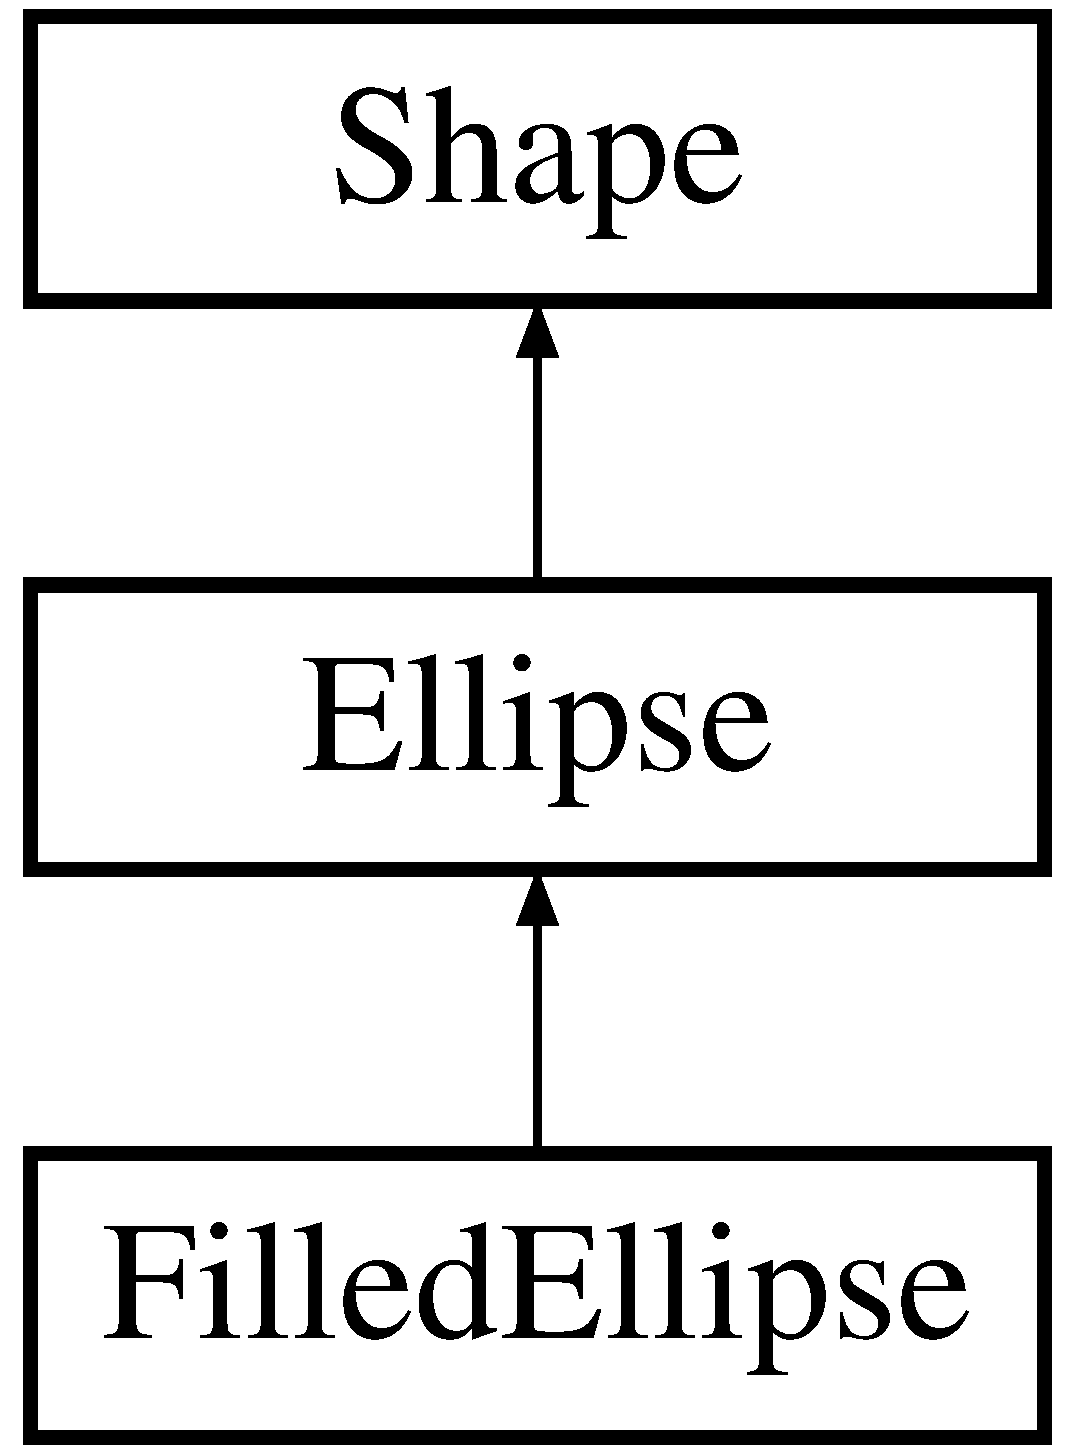
\includegraphics[height=3.000000cm]{classFilledEllipse}
\end{center}
\end{figure}
\subsection*{Public Member Functions}
\begin{DoxyCompactItemize}
\item 
\hyperlink{classFilledEllipse_aa3dfc1a2b1428966984ee92ee0e4a18b}{Filled\-Ellipse} (int in\-X1, int in\-Y1, int in\-X2, int in\-Y2, float c\mbox{[}3\mbox{]}, float b\mbox{[}3\mbox{]})
\item 
\hyperlink{classFilledEllipse_a46d02d99024ca857cb5e08187b2d265f}{$\sim$\-Filled\-Ellipse} ()
\item 
void \hyperlink{classFilledEllipse_a6010d7760f8418439ecdbcc1dcfe9b4c}{draw} () const 
\item 
bool \hyperlink{classFilledEllipse_a1b18f3c89f3d44a0d091b4a5a5890816}{contains} (int a, int b) const 
\item 
void \hyperlink{classFilledEllipse_a3fd1d3d0b506716399ec543a32a3c450}{move} (int x, int y)
\end{DoxyCompactItemize}
\subsection*{Additional Inherited Members}


\subsection{Detailed Description}
This is the \hyperlink{classFilledEllipse}{Filled\-Ellipse} Class. It inherits from the \hyperlink{classEllipse}{Ellipse} class. 

\subsection{Constructor \& Destructor Documentation}
\hypertarget{classFilledEllipse_aa3dfc1a2b1428966984ee92ee0e4a18b}{\index{Filled\-Ellipse@{Filled\-Ellipse}!Filled\-Ellipse@{Filled\-Ellipse}}
\index{Filled\-Ellipse@{Filled\-Ellipse}!FilledEllipse@{Filled\-Ellipse}}
\subsubsection[{Filled\-Ellipse}]{\setlength{\rightskip}{0pt plus 5cm}Filled\-Ellipse\-::\-Filled\-Ellipse (
\begin{DoxyParamCaption}
\item[{int}]{in\-X1, }
\item[{int}]{in\-Y1, }
\item[{int}]{in\-X2, }
\item[{int}]{in\-Y2, }
\item[{float}]{c\mbox{[}3\mbox{]}, }
\item[{float}]{b\mbox{[}3\mbox{]}}
\end{DoxyParamCaption}
)}}\label{classFilledEllipse_aa3dfc1a2b1428966984ee92ee0e4a18b}
\hyperlink{classFilledEllipse}{Filled\-Ellipse} constructor

\begin{DoxyAuthor}{Author}
Luke Videckis
\end{DoxyAuthor}
\begin{DoxyParagraph}{Description\-:}
This is the constructor for the \hyperlink{classFilledEllipse}{Filled\-Ellipse} class. It just updates the values for the class.
\end{DoxyParagraph}

\begin{DoxyParams}[1]{Parameters}
\mbox{\tt in}  & {\em in\-X1} & -\/ the x value of the down click \\
\hline
\mbox{\tt in}  & {\em in\-Y1} & -\/ the y value of the down click \\
\hline
\mbox{\tt in}  & {\em in\-X2} & -\/ the x value of the up click \\
\hline
\mbox{\tt in}  & {\em in\-Y2} & -\/ the y value of the up click \\
\hline
\mbox{\tt in}  & {\em c} & -\/ the float of R\-G\-B values for the color of the \hyperlink{classEllipse}{Ellipse} \\
\hline
\mbox{\tt in}  & {\em b} & -\/ the float of R\-G\-B values for the border of the \hyperlink{classEllipse}{Ellipse}\\
\hline
\end{DoxyParams}
\begin{DoxyReturn}{Returns}
nothing 
\end{DoxyReturn}
\hypertarget{classFilledEllipse_a46d02d99024ca857cb5e08187b2d265f}{\index{Filled\-Ellipse@{Filled\-Ellipse}!$\sim$\-Filled\-Ellipse@{$\sim$\-Filled\-Ellipse}}
\index{$\sim$\-Filled\-Ellipse@{$\sim$\-Filled\-Ellipse}!FilledEllipse@{Filled\-Ellipse}}
\subsubsection[{$\sim$\-Filled\-Ellipse}]{\setlength{\rightskip}{0pt plus 5cm}Filled\-Ellipse\-::$\sim$\-Filled\-Ellipse (
\begin{DoxyParamCaption}
{}
\end{DoxyParamCaption}
)}}\label{classFilledEllipse_a46d02d99024ca857cb5e08187b2d265f}
filled ellipse destructor

\begin{DoxyAuthor}{Author}
Luke Videckis
\end{DoxyAuthor}
\begin{DoxyParagraph}{Description\-:}
This is the destructor for the \hyperlink{classFilledEllipse}{Filled\-Ellipse} class. It doesn't do much.
\end{DoxyParagraph}
\begin{DoxyReturn}{Returns}
nothing 
\end{DoxyReturn}


\subsection{Member Function Documentation}
\hypertarget{classFilledEllipse_a1b18f3c89f3d44a0d091b4a5a5890816}{\index{Filled\-Ellipse@{Filled\-Ellipse}!contains@{contains}}
\index{contains@{contains}!FilledEllipse@{Filled\-Ellipse}}
\subsubsection[{contains}]{\setlength{\rightskip}{0pt plus 5cm}bool Filled\-Ellipse\-::contains (
\begin{DoxyParamCaption}
\item[{int}]{a, }
\item[{int}]{b}
\end{DoxyParamCaption}
) const\hspace{0.3cm}{\ttfamily [virtual]}}}\label{classFilledEllipse_a1b18f3c89f3d44a0d091b4a5a5890816}
filled ellipse contains function

\begin{DoxyAuthor}{Author}
Luke Videckis
\end{DoxyAuthor}
\begin{DoxyParagraph}{Description\-:}
This functions returns true if the click is inside the ellipse and false otherwise. It is exactly the same as the contains function for the ellipse class.
\end{DoxyParagraph}

\begin{DoxyParams}{Parameters}
{\em a} & -\/ the x value of the click to be checked \\
\hline
{\em b} & -\/ the y value of the click to be checked\\
\hline
\end{DoxyParams}
\begin{DoxyReturn}{Returns}
true if the click inside the ellipse 

false if the click is outside the ellipse 
\end{DoxyReturn}


Reimplemented from \hyperlink{classEllipse_a31b6310abda060741eb7033636709ce6}{Ellipse}.

\hypertarget{classFilledEllipse_a6010d7760f8418439ecdbcc1dcfe9b4c}{\index{Filled\-Ellipse@{Filled\-Ellipse}!draw@{draw}}
\index{draw@{draw}!FilledEllipse@{Filled\-Ellipse}}
\subsubsection[{draw}]{\setlength{\rightskip}{0pt plus 5cm}void Filled\-Ellipse\-::draw (
\begin{DoxyParamCaption}
{}
\end{DoxyParamCaption}
) const\hspace{0.3cm}{\ttfamily [virtual]}}}\label{classFilledEllipse_a6010d7760f8418439ecdbcc1dcfe9b4c}
filled ellipse draw function

\begin{DoxyAuthor}{Author}
Luke Videckis
\end{DoxyAuthor}
\begin{DoxyParagraph}{Description\-:}
This function draws an ellipse with a fill and border color.
\end{DoxyParagraph}
\begin{DoxyReturn}{Returns}
nothing 
\end{DoxyReturn}


Reimplemented from \hyperlink{classEllipse_a99c72122041b0523dc9227fc3e985179}{Ellipse}.

\hypertarget{classFilledEllipse_a3fd1d3d0b506716399ec543a32a3c450}{\index{Filled\-Ellipse@{Filled\-Ellipse}!move@{move}}
\index{move@{move}!FilledEllipse@{Filled\-Ellipse}}
\subsubsection[{move}]{\setlength{\rightskip}{0pt plus 5cm}void Filled\-Ellipse\-::move (
\begin{DoxyParamCaption}
\item[{int}]{x, }
\item[{int}]{y}
\end{DoxyParamCaption}
)\hspace{0.3cm}{\ttfamily [virtual]}}}\label{classFilledEllipse_a3fd1d3d0b506716399ec543a32a3c450}
filled ellipse move function

\begin{DoxyAuthor}{Author}
Jeffrey Ross
\end{DoxyAuthor}
\begin{DoxyParagraph}{Description\-:}
this function displaces the object on the xy axis' with the provided x and y value
\end{DoxyParagraph}
param\mbox{[}in\mbox{]} x -\/ amount to displace on x axis param\mbox{[}in\mbox{]} y -\/ amount to displace on y axis

\begin{DoxyReturn}{Returns}
nothing 
\end{DoxyReturn}


Reimplemented from \hyperlink{classEllipse_a7b536dcba1a231980299d2f309ab6fe0}{Ellipse}.



The documentation for this class was generated from the following files\-:\begin{DoxyCompactItemize}
\item 
\hyperlink{FilledEllipse_8h}{Filled\-Ellipse.\-h}\item 
\hyperlink{FilledEllipse_8cpp}{Filled\-Ellipse.\-cpp}\end{DoxyCompactItemize}

\hypertarget{classFilledRectangle}{\section{Filled\-Rectangle Class Reference}
\label{classFilledRectangle}\index{Filled\-Rectangle@{Filled\-Rectangle}}
}


This is the \hyperlink{classFilledRectangle}{Filled\-Rectangle} Class. It inherits from the \hyperlink{classRectangle}{Rectangle} class.  




{\ttfamily \#include $<$Filled\-Rectangle.\-h$>$}

Inheritance diagram for Filled\-Rectangle\-:\begin{figure}[H]
\begin{center}
\leavevmode
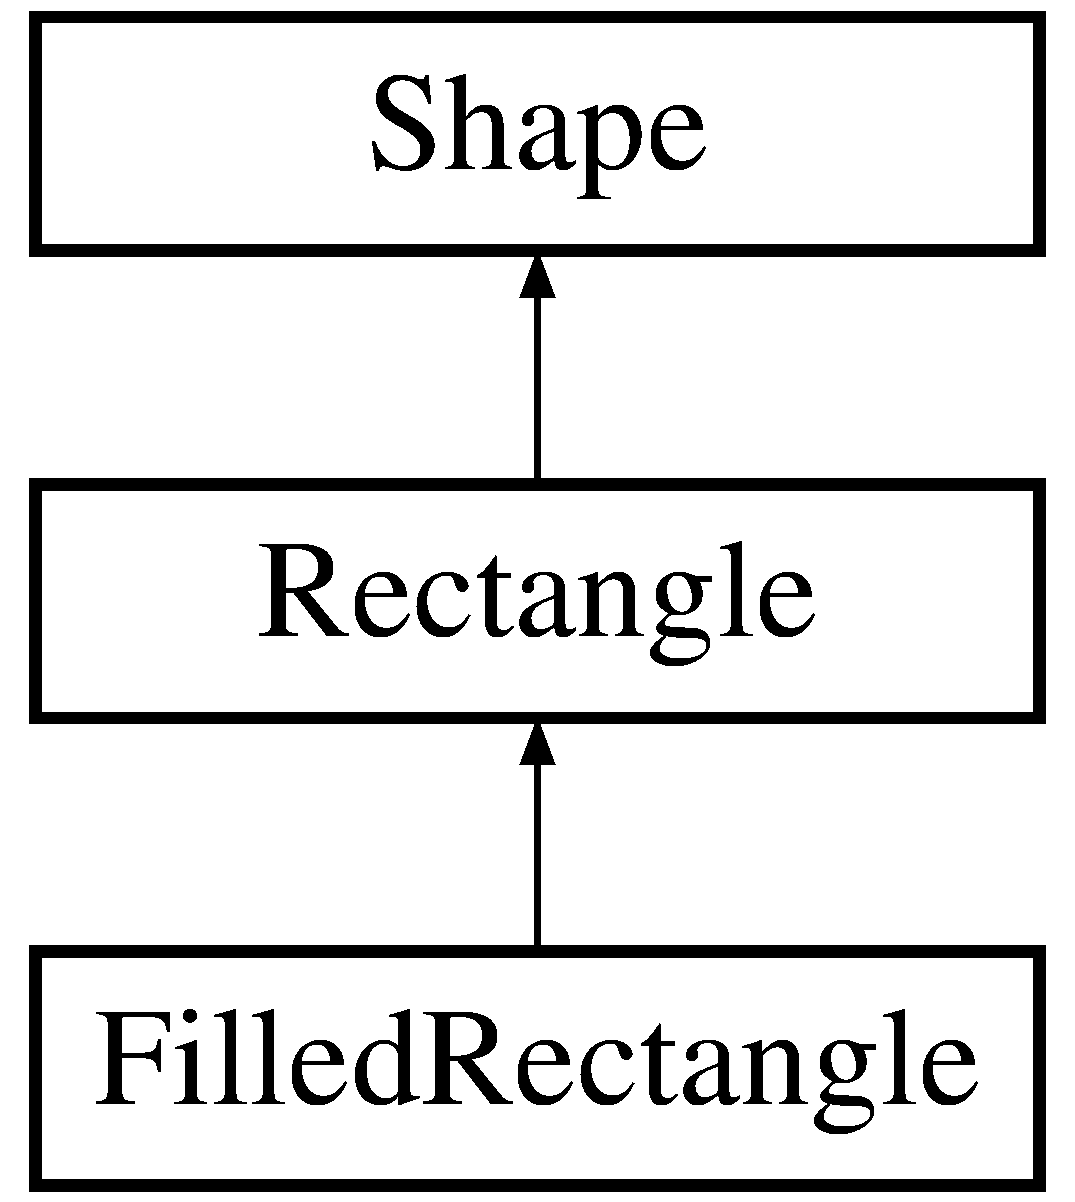
\includegraphics[height=3.000000cm]{classFilledRectangle}
\end{center}
\end{figure}
\subsection*{Public Member Functions}
\begin{DoxyCompactItemize}
\item 
\hyperlink{classFilledRectangle_af486107ac4b31342ab021e9953daa244}{Filled\-Rectangle} (int i1, int j1, int i2, int j2, float c\mbox{[}3\mbox{]}, float b\mbox{[}3\mbox{]})
\item 
\hyperlink{classFilledRectangle_a56e0054800fc14cf782591c19545e07b}{$\sim$\-Filled\-Rectangle} ()
\item 
void \hyperlink{classFilledRectangle_a49851c7d17a59e69c78e8957e25b5aec}{draw} () const 
\item 
bool \hyperlink{classFilledRectangle_a7db0492e684aee027407af324db12f5e}{contains} (int a, int b) const 
\item 
void \hyperlink{classFilledRectangle_acbf15e9451754a1ab873c97decf6718b}{move} (int x, int y)
\end{DoxyCompactItemize}
\subsection*{Additional Inherited Members}


\subsection{Detailed Description}
This is the \hyperlink{classFilledRectangle}{Filled\-Rectangle} Class. It inherits from the \hyperlink{classRectangle}{Rectangle} class. 

\subsection{Constructor \& Destructor Documentation}
\hypertarget{classFilledRectangle_af486107ac4b31342ab021e9953daa244}{\index{Filled\-Rectangle@{Filled\-Rectangle}!Filled\-Rectangle@{Filled\-Rectangle}}
\index{Filled\-Rectangle@{Filled\-Rectangle}!FilledRectangle@{Filled\-Rectangle}}
\subsubsection[{Filled\-Rectangle}]{\setlength{\rightskip}{0pt plus 5cm}Filled\-Rectangle\-::\-Filled\-Rectangle (
\begin{DoxyParamCaption}
\item[{int}]{i1, }
\item[{int}]{j1, }
\item[{int}]{i2, }
\item[{int}]{j2, }
\item[{float}]{c\mbox{[}3\mbox{]}, }
\item[{float}]{b\mbox{[}3\mbox{]}}
\end{DoxyParamCaption}
)}}\label{classFilledRectangle_af486107ac4b31342ab021e9953daa244}
filled rectangle constructor \hypertarget{classFilledRectangle_a56e0054800fc14cf782591c19545e07b}{\index{Filled\-Rectangle@{Filled\-Rectangle}!$\sim$\-Filled\-Rectangle@{$\sim$\-Filled\-Rectangle}}
\index{$\sim$\-Filled\-Rectangle@{$\sim$\-Filled\-Rectangle}!FilledRectangle@{Filled\-Rectangle}}
\subsubsection[{$\sim$\-Filled\-Rectangle}]{\setlength{\rightskip}{0pt plus 5cm}Filled\-Rectangle\-::$\sim$\-Filled\-Rectangle (
\begin{DoxyParamCaption}
{}
\end{DoxyParamCaption}
)}}\label{classFilledRectangle_a56e0054800fc14cf782591c19545e07b}
filled rectangle destructor

\begin{DoxyAuthor}{Author}
Luke Videckis
\end{DoxyAuthor}
\begin{DoxyParagraph}{Description\-:}
This is the destructor for the \hyperlink{classFilledRectangle}{Filled\-Rectangle} class.
\end{DoxyParagraph}
\begin{DoxyReturn}{Returns}
nothing 
\end{DoxyReturn}


\subsection{Member Function Documentation}
\hypertarget{classFilledRectangle_a7db0492e684aee027407af324db12f5e}{\index{Filled\-Rectangle@{Filled\-Rectangle}!contains@{contains}}
\index{contains@{contains}!FilledRectangle@{Filled\-Rectangle}}
\subsubsection[{contains}]{\setlength{\rightskip}{0pt plus 5cm}bool Filled\-Rectangle\-::contains (
\begin{DoxyParamCaption}
\item[{int}]{a, }
\item[{int}]{b}
\end{DoxyParamCaption}
) const\hspace{0.3cm}{\ttfamily [virtual]}}}\label{classFilledRectangle_a7db0492e684aee027407af324db12f5e}
filled rectangle contains function

\begin{DoxyAuthor}{Author}
Jeffrey Ross
\end{DoxyAuthor}
\begin{DoxyParagraph}{Description\-:}
a function that checks to see if the rectangle contains a certain (x,y) coordinate.
\end{DoxyParagraph}
\begin{DoxyReturn}{Returns}
true -\/ if it contains the coordinates 

false -\/ if it does not contain the coordinates 
\end{DoxyReturn}


Implements \hyperlink{classShape_abd90f6afcbacf45d1bcccc8225243101}{Shape}.

\hypertarget{classFilledRectangle_a49851c7d17a59e69c78e8957e25b5aec}{\index{Filled\-Rectangle@{Filled\-Rectangle}!draw@{draw}}
\index{draw@{draw}!FilledRectangle@{Filled\-Rectangle}}
\subsubsection[{draw}]{\setlength{\rightskip}{0pt plus 5cm}void Filled\-Rectangle\-::draw (
\begin{DoxyParamCaption}
{}
\end{DoxyParamCaption}
) const\hspace{0.3cm}{\ttfamily [virtual]}}}\label{classFilledRectangle_a49851c7d17a59e69c78e8957e25b5aec}
filled rectangle draw function

\begin{DoxyAuthor}{Author}
Jeffrey Ross
\end{DoxyAuthor}
\begin{DoxyParagraph}{Description\-:}
a function that prints the filled rectangle to the screen
\end{DoxyParagraph}
\begin{DoxyReturn}{Returns}
nothing 
\end{DoxyReturn}


Implements \hyperlink{classShape_a0d778013ae2532b958c8403155b36b7a}{Shape}.

\hypertarget{classFilledRectangle_acbf15e9451754a1ab873c97decf6718b}{\index{Filled\-Rectangle@{Filled\-Rectangle}!move@{move}}
\index{move@{move}!FilledRectangle@{Filled\-Rectangle}}
\subsubsection[{move}]{\setlength{\rightskip}{0pt plus 5cm}void Filled\-Rectangle\-::move (
\begin{DoxyParamCaption}
\item[{int}]{x, }
\item[{int}]{y}
\end{DoxyParamCaption}
)\hspace{0.3cm}{\ttfamily [virtual]}}}\label{classFilledRectangle_acbf15e9451754a1ab873c97decf6718b}
filled rectangle move function

\begin{DoxyAuthor}{Author}
Jeffrey Ross
\end{DoxyAuthor}
\begin{DoxyParagraph}{Description\-:}
this function displaces the object on the xy axis' with the provided x and y value
\end{DoxyParagraph}
param\mbox{[}in\mbox{]} x -\/ amount to displace on x axis param\mbox{[}in\mbox{]} y -\/ amount to displace on y axis

\begin{DoxyReturn}{Returns}
nothing 
\end{DoxyReturn}


Implements \hyperlink{classShape_a140551e1a4fc2c4d8cf8d2e01c5a5932}{Shape}.



The documentation for this class was generated from the following files\-:\begin{DoxyCompactItemize}
\item 
\hyperlink{FilledRectangle_8h}{Filled\-Rectangle.\-h}\item 
\hyperlink{FilledRectangle_8cpp}{Filled\-Rectangle.\-cpp}\end{DoxyCompactItemize}

\hypertarget{classLine}{\section{Line Class Reference}
\label{classLine}\index{Line@{Line}}
}


This is the \hyperlink{classLine}{Line} class. It inherits from the \hyperlink{classShape}{Shape} class.  




{\ttfamily \#include $<$line.\-h$>$}

Inheritance diagram for Line\-:\begin{figure}[H]
\begin{center}
\leavevmode
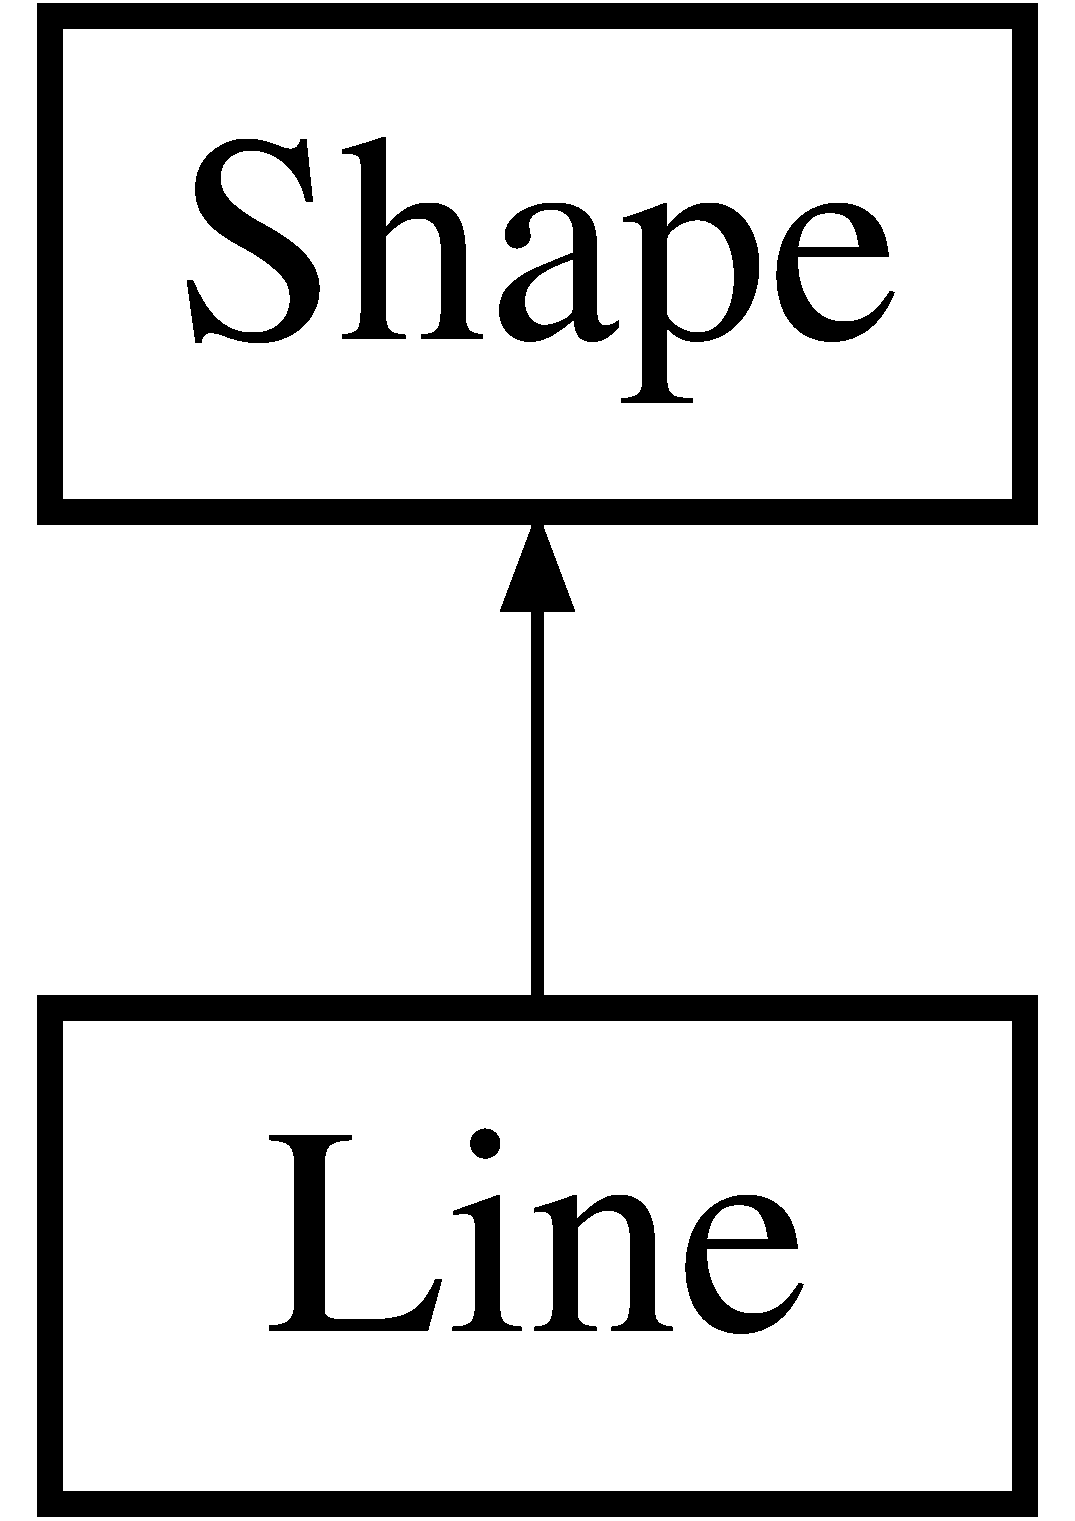
\includegraphics[height=2.000000cm]{classLine}
\end{center}
\end{figure}
\subsection*{Public Member Functions}
\begin{DoxyCompactItemize}
\item 
\hyperlink{classLine_afc1bfd0f0c5c94e78f7a157fdecae905}{Line} (int x1, int y1, int x2, int y2, float \hyperlink{classShape_a9f925188936af909e796807fc75c1501}{color}\mbox{[}3\mbox{]})
\item 
\hyperlink{classLine_aabe85f48d22d92b62257091f48174fac}{$\sim$\-Line} ()
\item 
void \hyperlink{classLine_ac54adb686a64dd9bd1701207a6cf2a83}{draw} () const 
\item 
bool \hyperlink{classLine_a0c1073cc62a7dc78b7f49bc776f40b40}{contains} (int a, int b) const 
\item 
void \hyperlink{classLine_a1dac74ba3a1c1770079dae9901e05af2}{move} (int x, int y)
\end{DoxyCompactItemize}
\subsection*{Additional Inherited Members}


\subsection{Detailed Description}
This is the \hyperlink{classLine}{Line} class. It inherits from the \hyperlink{classShape}{Shape} class. 

\subsection{Constructor \& Destructor Documentation}
\hypertarget{classLine_afc1bfd0f0c5c94e78f7a157fdecae905}{\index{Line@{Line}!Line@{Line}}
\index{Line@{Line}!Line@{Line}}
\subsubsection[{Line}]{\setlength{\rightskip}{0pt plus 5cm}Line\-::\-Line (
\begin{DoxyParamCaption}
\item[{int}]{x1, }
\item[{int}]{y1, }
\item[{int}]{x2, }
\item[{int}]{y2, }
\item[{float}]{color\mbox{[}3\mbox{]}}
\end{DoxyParamCaption}
)}}\label{classLine_afc1bfd0f0c5c94e78f7a157fdecae905}
line constructor

\begin{DoxyAuthor}{Author}
Luke Videckis
\end{DoxyAuthor}
\begin{DoxyParagraph}{Description\-:}
This is the constructor for the \hyperlink{classLine}{Line} class. It just updates the values for the class. (wow, that's awesome!)
\end{DoxyParagraph}

\begin{DoxyParams}[1]{Parameters}
\mbox{\tt in}  & {\em x1} & -\/ the x value of the down click \\
\hline
\mbox{\tt in}  & {\em y1} & -\/ the y value of the down click \\
\hline
\mbox{\tt in}  & {\em x2} & -\/ the x value of the up click \\
\hline
\mbox{\tt in}  & {\em y2} & -\/ the y value of the up click \\
\hline
\mbox{\tt in}  & {\em color} & -\/ the float of R\-G\-B values for the line\\
\hline
\end{DoxyParams}
\begin{DoxyReturn}{Returns}
nothing 
\end{DoxyReturn}
\hypertarget{classLine_aabe85f48d22d92b62257091f48174fac}{\index{Line@{Line}!$\sim$\-Line@{$\sim$\-Line}}
\index{$\sim$\-Line@{$\sim$\-Line}!Line@{Line}}
\subsubsection[{$\sim$\-Line}]{\setlength{\rightskip}{0pt plus 5cm}Line\-::$\sim$\-Line (
\begin{DoxyParamCaption}
{}
\end{DoxyParamCaption}
)}}\label{classLine_aabe85f48d22d92b62257091f48174fac}
line destructor

\begin{DoxyAuthor}{Author}
Luke Videckis
\end{DoxyAuthor}
\begin{DoxyParagraph}{Description\-:}
This is the destructor for the \hyperlink{classLine}{Line} class. It does absolutely nothing. Nice.
\end{DoxyParagraph}
\begin{DoxyReturn}{Returns}
nothing 
\end{DoxyReturn}


\subsection{Member Function Documentation}
\hypertarget{classLine_a0c1073cc62a7dc78b7f49bc776f40b40}{\index{Line@{Line}!contains@{contains}}
\index{contains@{contains}!Line@{Line}}
\subsubsection[{contains}]{\setlength{\rightskip}{0pt plus 5cm}bool Line\-::contains (
\begin{DoxyParamCaption}
\item[{int}]{a, }
\item[{int}]{c}
\end{DoxyParamCaption}
) const\hspace{0.3cm}{\ttfamily [virtual]}}}\label{classLine_a0c1073cc62a7dc78b7f49bc776f40b40}
line contains function

\begin{DoxyAuthor}{Author}
Luke Videckis
\end{DoxyAuthor}
\begin{DoxyParagraph}{Description\-:}
This functions returns true if the click is near the line and false otherwise. Near the line means the click is anywhere between 30 pixels above or below the line.
\end{DoxyParagraph}

\begin{DoxyParams}[1]{Parameters}
\mbox{\tt in}  & {\em a} & -\/ the x value of the click to be checked \\
\hline
\mbox{\tt in}  & {\em c} & -\/ the y value of the click to be checked\\
\hline
\end{DoxyParams}
\begin{DoxyReturn}{Returns}
true if the click is near the line 

false if the click is not near the line 
\end{DoxyReturn}


Implements \hyperlink{classShape_abd90f6afcbacf45d1bcccc8225243101}{Shape}.

\hypertarget{classLine_ac54adb686a64dd9bd1701207a6cf2a83}{\index{Line@{Line}!draw@{draw}}
\index{draw@{draw}!Line@{Line}}
\subsubsection[{draw}]{\setlength{\rightskip}{0pt plus 5cm}void Line\-::draw (
\begin{DoxyParamCaption}
{}
\end{DoxyParamCaption}
) const\hspace{0.3cm}{\ttfamily [virtual]}}}\label{classLine_ac54adb686a64dd9bd1701207a6cf2a83}
line draw function

\begin{DoxyAuthor}{Author}
Luke Videckis
\end{DoxyAuthor}
\begin{DoxyParagraph}{Description\-:}
This function draws a line (oooo spicy)
\end{DoxyParagraph}
\begin{DoxyReturn}{Returns}
nothing 
\end{DoxyReturn}


Implements \hyperlink{classShape_a0d778013ae2532b958c8403155b36b7a}{Shape}.

\hypertarget{classLine_a1dac74ba3a1c1770079dae9901e05af2}{\index{Line@{Line}!move@{move}}
\index{move@{move}!Line@{Line}}
\subsubsection[{move}]{\setlength{\rightskip}{0pt plus 5cm}void Line\-::move (
\begin{DoxyParamCaption}
\item[{int}]{x, }
\item[{int}]{y}
\end{DoxyParamCaption}
)\hspace{0.3cm}{\ttfamily [virtual]}}}\label{classLine_a1dac74ba3a1c1770079dae9901e05af2}
line move function

\begin{DoxyAuthor}{Author}
Jeffrey Ross
\end{DoxyAuthor}
\begin{DoxyParagraph}{Description\-:}
this function displaces the object on the xy axis' with the provided x and y value
\end{DoxyParagraph}
param\mbox{[}in\mbox{]} x -\/ amount to displace on x axis param\mbox{[}in\mbox{]} y -\/ amount to displace on y axis

\begin{DoxyReturn}{Returns}
nothing 
\end{DoxyReturn}


Implements \hyperlink{classShape_a140551e1a4fc2c4d8cf8d2e01c5a5932}{Shape}.



The documentation for this class was generated from the following files\-:\begin{DoxyCompactItemize}
\item 
\hyperlink{line_8h}{line.\-h}\item 
\hyperlink{line_8cpp}{line.\-cpp}\end{DoxyCompactItemize}

\hypertarget{classRectangle}{\section{Rectangle Class Reference}
\label{classRectangle}\index{Rectangle@{Rectangle}}
}


This is the \hyperlink{classRectangle}{Rectangle} Class. It inherits from the \hyperlink{classShape}{Shape} class.  




{\ttfamily \#include $<$rectangle.\-h$>$}

Inheritance diagram for Rectangle\-:\begin{figure}[H]
\begin{center}
\leavevmode
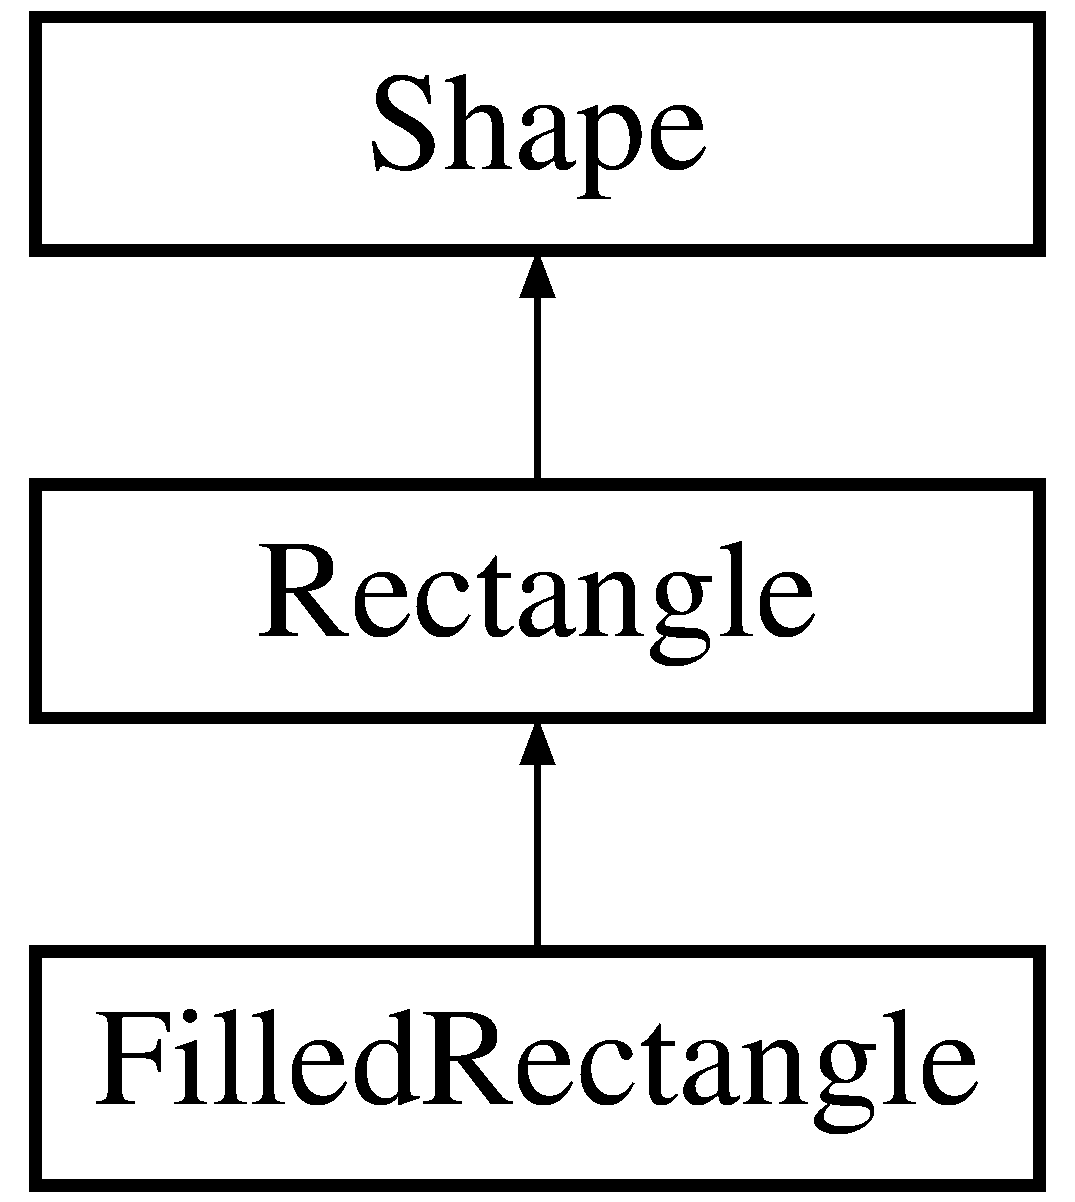
\includegraphics[height=3.000000cm]{classRectangle}
\end{center}
\end{figure}
\subsection*{Public Member Functions}
\begin{DoxyCompactItemize}
\item 
\hyperlink{classRectangle_adf0964454431d23ef36abea2496d587e}{Rectangle} (int i1, int j1, int i2, int j2, float c\mbox{[}3\mbox{]}, bool pal)
\item 
\hyperlink{classRectangle_a494c076b13aadf26efdce07d23c61ddd}{$\sim$\-Rectangle} ()
\item 
void \hyperlink{classRectangle_af3b5f195986cdf6c5b5df95fa9ab22b8}{draw} () const 
\item 
bool \hyperlink{classRectangle_a763094105c015cce727a486baff1dfaf}{contains} (int a, int b) const 
\item 
void \hyperlink{classRectangle_a5723f7551b73038c4aadf2fa833f7fcd}{is\-Pallete} ()
\item 
void \hyperlink{classRectangle_a3cfcca33879bd4cd31ed738578eca79e}{move} (int x, int y)
\end{DoxyCompactItemize}
\subsection*{Additional Inherited Members}


\subsection{Detailed Description}
This is the \hyperlink{classRectangle}{Rectangle} Class. It inherits from the \hyperlink{classShape}{Shape} class. 

\subsection{Constructor \& Destructor Documentation}
\hypertarget{classRectangle_adf0964454431d23ef36abea2496d587e}{\index{Rectangle@{Rectangle}!Rectangle@{Rectangle}}
\index{Rectangle@{Rectangle}!Rectangle@{Rectangle}}
\subsubsection[{Rectangle}]{\setlength{\rightskip}{0pt plus 5cm}Rectangle\-::\-Rectangle (
\begin{DoxyParamCaption}
\item[{int}]{i1, }
\item[{int}]{j1, }
\item[{int}]{i2, }
\item[{int}]{j2, }
\item[{float}]{c\mbox{[}3\mbox{]}, }
\item[{bool}]{pal}
\end{DoxyParamCaption}
)}}\label{classRectangle_adf0964454431d23ef36abea2496d587e}
rectangle constructor \hypertarget{classRectangle_a494c076b13aadf26efdce07d23c61ddd}{\index{Rectangle@{Rectangle}!$\sim$\-Rectangle@{$\sim$\-Rectangle}}
\index{$\sim$\-Rectangle@{$\sim$\-Rectangle}!Rectangle@{Rectangle}}
\subsubsection[{$\sim$\-Rectangle}]{\setlength{\rightskip}{0pt plus 5cm}Rectangle\-::$\sim$\-Rectangle (
\begin{DoxyParamCaption}
{}
\end{DoxyParamCaption}
)}}\label{classRectangle_a494c076b13aadf26efdce07d23c61ddd}
rectangle destructor 

\subsection{Member Function Documentation}
\hypertarget{classRectangle_a763094105c015cce727a486baff1dfaf}{\index{Rectangle@{Rectangle}!contains@{contains}}
\index{contains@{contains}!Rectangle@{Rectangle}}
\subsubsection[{contains}]{\setlength{\rightskip}{0pt plus 5cm}bool Rectangle\-::contains (
\begin{DoxyParamCaption}
\item[{int}]{a, }
\item[{int}]{b}
\end{DoxyParamCaption}
) const\hspace{0.3cm}{\ttfamily [virtual]}}}\label{classRectangle_a763094105c015cce727a486baff1dfaf}
rectangle contains function 

Implements \hyperlink{classShape_abd90f6afcbacf45d1bcccc8225243101}{Shape}.

\hypertarget{classRectangle_af3b5f195986cdf6c5b5df95fa9ab22b8}{\index{Rectangle@{Rectangle}!draw@{draw}}
\index{draw@{draw}!Rectangle@{Rectangle}}
\subsubsection[{draw}]{\setlength{\rightskip}{0pt plus 5cm}void Rectangle\-::draw (
\begin{DoxyParamCaption}
{}
\end{DoxyParamCaption}
) const\hspace{0.3cm}{\ttfamily [virtual]}}}\label{classRectangle_af3b5f195986cdf6c5b5df95fa9ab22b8}
rectangle draw function 

Implements \hyperlink{classShape_a0d778013ae2532b958c8403155b36b7a}{Shape}.

\hypertarget{classRectangle_a5723f7551b73038c4aadf2fa833f7fcd}{\index{Rectangle@{Rectangle}!is\-Pallete@{is\-Pallete}}
\index{is\-Pallete@{is\-Pallete}!Rectangle@{Rectangle}}
\subsubsection[{is\-Pallete}]{\setlength{\rightskip}{0pt plus 5cm}void Rectangle\-::is\-Pallete (
\begin{DoxyParamCaption}
{}
\end{DoxyParamCaption}
)}}\label{classRectangle_a5723f7551b73038c4aadf2fa833f7fcd}
rectangle function to check if its in the palette \hypertarget{classRectangle_a3cfcca33879bd4cd31ed738578eca79e}{\index{Rectangle@{Rectangle}!move@{move}}
\index{move@{move}!Rectangle@{Rectangle}}
\subsubsection[{move}]{\setlength{\rightskip}{0pt plus 5cm}void Rectangle\-::move (
\begin{DoxyParamCaption}
\item[{int}]{x, }
\item[{int}]{y}
\end{DoxyParamCaption}
)\hspace{0.3cm}{\ttfamily [virtual]}}}\label{classRectangle_a3cfcca33879bd4cd31ed738578eca79e}
rectangle move function 

Implements \hyperlink{classShape_a140551e1a4fc2c4d8cf8d2e01c5a5932}{Shape}.



The documentation for this class was generated from the following files\-:\begin{DoxyCompactItemize}
\item 
\hyperlink{rectangle_8h}{rectangle.\-h}\item 
\hyperlink{rectangle_8cpp}{rectangle.\-cpp}\end{DoxyCompactItemize}

\hypertarget{classShape}{\section{Shape Class Reference}
\label{classShape}\index{Shape@{Shape}}
}


This is the \hyperlink{classShape}{Shape} class.  




{\ttfamily \#include $<$shape.\-h$>$}

Inheritance diagram for Shape\-:\begin{figure}[H]
\begin{center}
\leavevmode
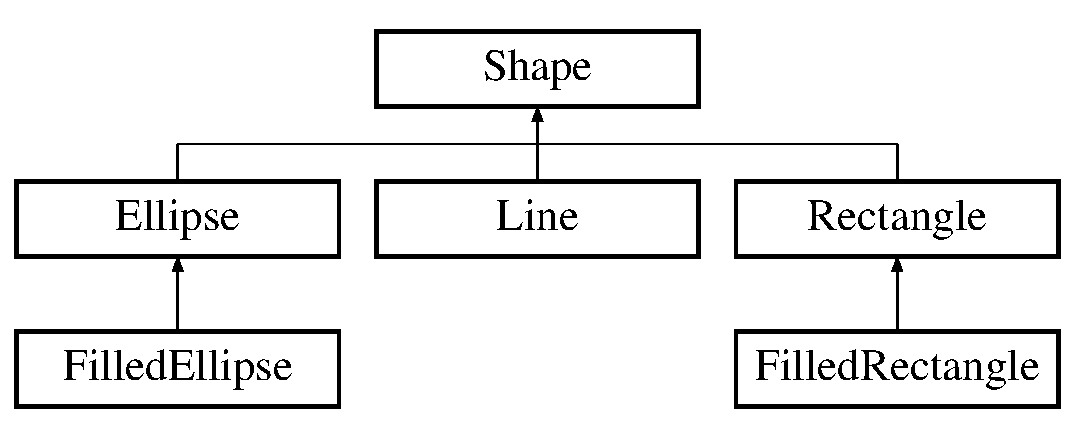
\includegraphics[height=3.000000cm]{classShape}
\end{center}
\end{figure}
\subsection*{Public Member Functions}
\begin{DoxyCompactItemize}
\item 
virtual \hyperlink{classShape_ac3b9fc48965274893f25b18aa14ba665}{$\sim$\-Shape} ()
\item 
virtual void \hyperlink{classShape_a0d778013ae2532b958c8403155b36b7a}{draw} () const =0
\item 
virtual bool \hyperlink{classShape_abd90f6afcbacf45d1bcccc8225243101}{contains} (int a, int b) const =0
\item 
virtual void \hyperlink{classShape_a140551e1a4fc2c4d8cf8d2e01c5a5932}{move} (int x, int y)=0
\end{DoxyCompactItemize}
\subsection*{Public Attributes}
\begin{DoxyCompactItemize}
\item 
float \hyperlink{classShape_a9f925188936af909e796807fc75c1501}{color} \mbox{[}3\mbox{]}
\item 
float \hyperlink{classShape_ac4439415a7e663a7088fe36244cefaca}{border} \mbox{[}3\mbox{]}
\item 
std\-::vector$<$ int $>$ \hyperlink{classShape_affa8864633ce066ea626eb50fb4d7584}{display\-Shapes}
\end{DoxyCompactItemize}


\subsection{Detailed Description}
This is the \hyperlink{classShape}{Shape} class. 

\subsection{Constructor \& Destructor Documentation}
\hypertarget{classShape_ac3b9fc48965274893f25b18aa14ba665}{\index{Shape@{Shape}!$\sim$\-Shape@{$\sim$\-Shape}}
\index{$\sim$\-Shape@{$\sim$\-Shape}!Shape@{Shape}}
\subsubsection[{$\sim$\-Shape}]{\setlength{\rightskip}{0pt plus 5cm}virtual Shape\-::$\sim$\-Shape (
\begin{DoxyParamCaption}
{}
\end{DoxyParamCaption}
)\hspace{0.3cm}{\ttfamily [inline]}, {\ttfamily [virtual]}}}\label{classShape_ac3b9fc48965274893f25b18aa14ba665}
\hyperlink{classShape}{Shape} destructor 

\subsection{Member Function Documentation}
\hypertarget{classShape_abd90f6afcbacf45d1bcccc8225243101}{\index{Shape@{Shape}!contains@{contains}}
\index{contains@{contains}!Shape@{Shape}}
\subsubsection[{contains}]{\setlength{\rightskip}{0pt plus 5cm}virtual bool Shape\-::contains (
\begin{DoxyParamCaption}
\item[{int}]{a, }
\item[{int}]{b}
\end{DoxyParamCaption}
) const\hspace{0.3cm}{\ttfamily [pure virtual]}}}\label{classShape_abd90f6afcbacf45d1bcccc8225243101}
shape contains function 

Implemented in \hyperlink{classRectangle_a763094105c015cce727a486baff1dfaf}{Rectangle}, \hyperlink{classEllipse_a31b6310abda060741eb7033636709ce6}{Ellipse}, \hyperlink{classFilledEllipse_a1b18f3c89f3d44a0d091b4a5a5890816}{Filled\-Ellipse}, \hyperlink{classFilledRectangle_a7db0492e684aee027407af324db12f5e}{Filled\-Rectangle}, and \hyperlink{classLine_a0c1073cc62a7dc78b7f49bc776f40b40}{Line}.

\hypertarget{classShape_a0d778013ae2532b958c8403155b36b7a}{\index{Shape@{Shape}!draw@{draw}}
\index{draw@{draw}!Shape@{Shape}}
\subsubsection[{draw}]{\setlength{\rightskip}{0pt plus 5cm}virtual void Shape\-::draw (
\begin{DoxyParamCaption}
{}
\end{DoxyParamCaption}
) const\hspace{0.3cm}{\ttfamily [pure virtual]}}}\label{classShape_a0d778013ae2532b958c8403155b36b7a}
shape draw function 

Implemented in \hyperlink{classRectangle_af3b5f195986cdf6c5b5df95fa9ab22b8}{Rectangle}, \hyperlink{classEllipse_a99c72122041b0523dc9227fc3e985179}{Ellipse}, \hyperlink{classFilledEllipse_a6010d7760f8418439ecdbcc1dcfe9b4c}{Filled\-Ellipse}, \hyperlink{classFilledRectangle_a49851c7d17a59e69c78e8957e25b5aec}{Filled\-Rectangle}, and \hyperlink{classLine_ac54adb686a64dd9bd1701207a6cf2a83}{Line}.

\hypertarget{classShape_a140551e1a4fc2c4d8cf8d2e01c5a5932}{\index{Shape@{Shape}!move@{move}}
\index{move@{move}!Shape@{Shape}}
\subsubsection[{move}]{\setlength{\rightskip}{0pt plus 5cm}virtual void Shape\-::move (
\begin{DoxyParamCaption}
\item[{int}]{x, }
\item[{int}]{y}
\end{DoxyParamCaption}
)\hspace{0.3cm}{\ttfamily [pure virtual]}}}\label{classShape_a140551e1a4fc2c4d8cf8d2e01c5a5932}
shape move function 

Implemented in \hyperlink{classRectangle_a3cfcca33879bd4cd31ed738578eca79e}{Rectangle}, \hyperlink{classEllipse_a7b536dcba1a231980299d2f309ab6fe0}{Ellipse}, \hyperlink{classFilledEllipse_a3fd1d3d0b506716399ec543a32a3c450}{Filled\-Ellipse}, \hyperlink{classFilledRectangle_acbf15e9451754a1ab873c97decf6718b}{Filled\-Rectangle}, and \hyperlink{classLine_a1dac74ba3a1c1770079dae9901e05af2}{Line}.



\subsection{Member Data Documentation}
\hypertarget{classShape_ac4439415a7e663a7088fe36244cefaca}{\index{Shape@{Shape}!border@{border}}
\index{border@{border}!Shape@{Shape}}
\subsubsection[{border}]{\setlength{\rightskip}{0pt plus 5cm}float Shape\-::border\mbox{[}3\mbox{]}}}\label{classShape_ac4439415a7e663a7088fe36244cefaca}
border color \hypertarget{classShape_a9f925188936af909e796807fc75c1501}{\index{Shape@{Shape}!color@{color}}
\index{color@{color}!Shape@{Shape}}
\subsubsection[{color}]{\setlength{\rightskip}{0pt plus 5cm}float Shape\-::color\mbox{[}3\mbox{]}}}\label{classShape_a9f925188936af909e796807fc75c1501}
fill color \hypertarget{classShape_affa8864633ce066ea626eb50fb4d7584}{\index{Shape@{Shape}!display\-Shapes@{display\-Shapes}}
\index{display\-Shapes@{display\-Shapes}!Shape@{Shape}}
\subsubsection[{display\-Shapes}]{\setlength{\rightskip}{0pt plus 5cm}std\-::vector$<$int$>$ Shape\-::display\-Shapes}}\label{classShape_affa8864633ce066ea626eb50fb4d7584}
list of ints which tell what shape it is 

The documentation for this class was generated from the following file\-:\begin{DoxyCompactItemize}
\item 
\hyperlink{shape_8h}{shape.\-h}\end{DoxyCompactItemize}

\chapter{File Documentation}
\hypertarget{ellipse_8cpp}{\section{ellipse.\-cpp File Reference}
\label{ellipse_8cpp}\index{ellipse.\-cpp@{ellipse.\-cpp}}
}
{\ttfamily \#include \char`\"{}ellipse.\-h\char`\"{}}\\*
{\ttfamily \#include $<$cmath$>$}\\*

\hypertarget{ellipse_8h}{\section{ellipse.\-h File Reference}
\label{ellipse_8h}\index{ellipse.\-h@{ellipse.\-h}}
}
{\ttfamily \#include $<$G\-L/freeglut.\-h$>$}\\*
{\ttfamily \#include \char`\"{}shape.\-h\char`\"{}}\\*
\subsection*{Classes}
\begin{DoxyCompactItemize}
\item 
class \hyperlink{classEllipse}{Ellipse}
\begin{DoxyCompactList}\small\item\em This is the \hyperlink{classEllipse}{Ellipse} Class. It inherits from the \hyperlink{classShape}{Shape} class. \end{DoxyCompactList}\end{DoxyCompactItemize}

\hypertarget{FilledEllipse_8cpp}{\section{Filled\-Ellipse.\-cpp File Reference}
\label{FilledEllipse_8cpp}\index{Filled\-Ellipse.\-cpp@{Filled\-Ellipse.\-cpp}}
}
{\ttfamily \#include \char`\"{}Filled\-Ellipse.\-h\char`\"{}}\\*
{\ttfamily \#include $<$cmath$>$}\\*

\hypertarget{FilledEllipse_8h}{\section{Filled\-Ellipse.\-h File Reference}
\label{FilledEllipse_8h}\index{Filled\-Ellipse.\-h@{Filled\-Ellipse.\-h}}
}
{\ttfamily \#include \char`\"{}ellipse.\-h\char`\"{}}\\*
\subsection*{Classes}
\begin{DoxyCompactItemize}
\item 
class \hyperlink{classFilledEllipse}{Filled\-Ellipse}
\begin{DoxyCompactList}\small\item\em This is the \hyperlink{classFilledEllipse}{Filled\-Ellipse} Class. It inherits from the \hyperlink{classEllipse}{Ellipse} class. \end{DoxyCompactList}\end{DoxyCompactItemize}

\hypertarget{FilledRectangle_8cpp}{\section{Filled\-Rectangle.\-cpp File Reference}
\label{FilledRectangle_8cpp}\index{Filled\-Rectangle.\-cpp@{Filled\-Rectangle.\-cpp}}
}
{\ttfamily \#include \char`\"{}Filled\-Rectangle.\-h\char`\"{}}\\*

\hypertarget{FilledRectangle_8h}{\section{Filled\-Rectangle.\-h File Reference}
\label{FilledRectangle_8h}\index{Filled\-Rectangle.\-h@{Filled\-Rectangle.\-h}}
}
{\ttfamily \#include \char`\"{}rectangle.\-h\char`\"{}}\\*
\subsection*{Classes}
\begin{DoxyCompactItemize}
\item 
class \hyperlink{classFilledRectangle}{Filled\-Rectangle}
\begin{DoxyCompactList}\small\item\em This is the \hyperlink{classFilledRectangle}{Filled\-Rectangle} Class. It inherits from the \hyperlink{classRectangle}{Rectangle} class. \end{DoxyCompactList}\end{DoxyCompactItemize}

\hypertarget{functions_8cpp}{\section{functions.\-cpp File Reference}
\label{functions_8cpp}\index{functions.\-cpp@{functions.\-cpp}}
}
{\ttfamily \#include $<$vector$>$}\\*
{\ttfamily \#include $<$cmath$>$}\\*
{\ttfamily \#include \char`\"{}functions.\-h\char`\"{}}\\*
{\ttfamily \#include \char`\"{}rectangle.\-h\char`\"{}}\\*
{\ttfamily \#include \char`\"{}ellipse.\-h\char`\"{}}\\*
{\ttfamily \#include \char`\"{}line.\-h\char`\"{}}\\*
{\ttfamily \#include \char`\"{}Filled\-Ellipse.\-h\char`\"{}}\\*
{\ttfamily \#include \char`\"{}Filled\-Rectangle.\-h\char`\"{}}\\*
\subsection*{Macros}
\begin{DoxyCompactItemize}
\item 
\#define \hyperlink{functions_8cpp_a8714238ce6eefa25f0f2db2b8caf29bf}{side}~40
\item 
\#define \hyperlink{functions_8cpp_a03237f39b55a602a065bfc72285557dc}{escape}~27
\end{DoxyCompactItemize}
\subsection*{Functions}
\begin{DoxyCompactItemize}
\item 
void \hyperlink{functions_8cpp_a1e5b20fed15743656bb6d2e6a6ea6269}{display} ()
\item 
void \hyperlink{functions_8cpp_aef7ba2f69afb2d954545f64c7fe24b14}{keyboard} (unsigned char key, int x, int y)
\item 
void \hyperlink{functions_8cpp_a125707cf235695f4eb006113f0c01265}{mouse\-Click} (int button, int state, int x, int y)
\item 
void \hyperlink{functions_8cpp_acc1ffe65e6869931318610cae7210078}{reshape} (int w, int h)
\item 
void \hyperlink{functions_8cpp_a4827868fe4bb8ea06d7c613259488b8d}{reshape\-Callback\-Name} (const int width, const int height)
\item 
void \hyperlink{functions_8cpp_ac67d6f71ce80edfed6148387d2dfc487}{print\-Palette} (int action, \hyperlink{structcurrentProperties}{current\-Properties} $\ast$curr)
\item 
void \hyperlink{functions_8cpp_a2ed838fa7a4a7be7950f11964b23a44e}{check\-Palette} (int x, int y, float(\&rtcolor)\mbox{[}3\mbox{]})
\item 
vector$<$ \hyperlink{classShape}{Shape} $\ast$ $>$ \hyperlink{functions_8cpp_aaba9e1b6d4a6c937669cc453b8c00290}{make\-Palette} ()
\item 
bool \hyperlink{functions_8cpp_a21e7194c7f7e8dee54e1fdb8ed206f4b}{edit\-Shapes} (int action, \hyperlink{classShape}{Shape} $\ast$temp, int x, int y)
\end{DoxyCompactItemize}


\subsection{Macro Definition Documentation}
\hypertarget{functions_8cpp_a03237f39b55a602a065bfc72285557dc}{\index{functions.\-cpp@{functions.\-cpp}!escape@{escape}}
\index{escape@{escape}!functions.cpp@{functions.\-cpp}}
\subsubsection[{escape}]{\setlength{\rightskip}{0pt plus 5cm}\#define escape~27}}\label{functions_8cpp_a03237f39b55a602a065bfc72285557dc}
this is used to know when the escape key is being pressed \hypertarget{functions_8cpp_a8714238ce6eefa25f0f2db2b8caf29bf}{\index{functions.\-cpp@{functions.\-cpp}!side@{side}}
\index{side@{side}!functions.cpp@{functions.\-cpp}}
\subsubsection[{side}]{\setlength{\rightskip}{0pt plus 5cm}\#define side~40}}\label{functions_8cpp_a8714238ce6eefa25f0f2db2b8caf29bf}
this makes the side length of a palette square 40 pixels 

\subsection{Function Documentation}
\hypertarget{functions_8cpp_a2ed838fa7a4a7be7950f11964b23a44e}{\index{functions.\-cpp@{functions.\-cpp}!check\-Palette@{check\-Palette}}
\index{check\-Palette@{check\-Palette}!functions.cpp@{functions.\-cpp}}
\subsubsection[{check\-Palette}]{\setlength{\rightskip}{0pt plus 5cm}void check\-Palette (
\begin{DoxyParamCaption}
\item[{int}]{x, }
\item[{int}]{y, }
\item[{float(\&)}]{rtcolor\mbox{[}3\mbox{]}}
\end{DoxyParamCaption}
)}}\label{functions_8cpp_a2ed838fa7a4a7be7950f11964b23a44e}
\begin{DoxyAuthor}{Author}
Jeffrey Ross
\end{DoxyAuthor}
\begin{DoxyParagraph}{Description\-:}
this function goes through a vector containing all rectangles of the palette, checking to see if they contain the passed x and y values. if the rectangle in the palette contains the coordinates, it will change the array of current colors or will change the next shape to be drawn. (shape portion not yet added)
\end{DoxyParagraph}

\begin{DoxyParams}[1]{Parameters}
\mbox{\tt in}  & {\em x} & -\/ coordinate to be checked \\
\hline
\mbox{\tt in}  & {\em y} & -\/ coordinate to be checked \\
\hline
\mbox{\tt in}  & {\em rtcolor} & -\/ an array containing R\-G\-B values for current color.\\
\hline
\end{DoxyParams}
\begin{DoxyReturn}{Returns}
-\/ nothing 
\end{DoxyReturn}
\hypertarget{functions_8cpp_a1e5b20fed15743656bb6d2e6a6ea6269}{\index{functions.\-cpp@{functions.\-cpp}!display@{display}}
\index{display@{display}!functions.cpp@{functions.\-cpp}}
\subsubsection[{display}]{\setlength{\rightskip}{0pt plus 5cm}void display (
\begin{DoxyParamCaption}
{}
\end{DoxyParamCaption}
)}}\label{functions_8cpp_a1e5b20fed15743656bb6d2e6a6ea6269}
\begin{DoxyAuthor}{Author}
Luke Videckis
\end{DoxyAuthor}
\begin{DoxyParagraph}{Description\-:}
This function will print the palette along with all the shapes drawn
\end{DoxyParagraph}
\begin{DoxyReturn}{Returns}
nothing 
\end{DoxyReturn}
\hypertarget{functions_8cpp_a21e7194c7f7e8dee54e1fdb8ed206f4b}{\index{functions.\-cpp@{functions.\-cpp}!edit\-Shapes@{edit\-Shapes}}
\index{edit\-Shapes@{edit\-Shapes}!functions.cpp@{functions.\-cpp}}
\subsubsection[{edit\-Shapes}]{\setlength{\rightskip}{0pt plus 5cm}bool edit\-Shapes (
\begin{DoxyParamCaption}
\item[{int}]{action, }
\item[{{\bf Shape} $\ast$}]{temp, }
\item[{int}]{x, }
\item[{int}]{y}
\end{DoxyParamCaption}
)}}\label{functions_8cpp_a21e7194c7f7e8dee54e1fdb8ed206f4b}
\begin{DoxyAuthor}{Author}
Jeffrey Ross
\end{DoxyAuthor}
\begin{DoxyParagraph}{Description\-:}
This function maintains all the shapes that are being displayed to the screen. It stores all the shapes in a vector and acts upon them accordingly based on the action that is passed in. It can add new shapes, print all the shapes, delete one or all shapes, and check if any shapes contain an (x,y) coordinate.
\end{DoxyParagraph}

\begin{DoxyParams}[1]{Parameters}
\mbox{\tt in}  & {\em temp} & -\/ pointer to a shape to be added \\
\hline
\mbox{\tt in}  & {\em action} & -\/ represents what action to take \\
\hline
\mbox{\tt in}  & {\em x} & -\/ x coordinate to be operated on \\
\hline
\mbox{\tt in}  & {\em y} & -\/ y coordinate to be operated on\\
\hline
\end{DoxyParams}
\begin{DoxyReturn}{Returns}
true if it contains an (x,y) coordinate 
\end{DoxyReturn}
\hypertarget{functions_8cpp_aef7ba2f69afb2d954545f64c7fe24b14}{\index{functions.\-cpp@{functions.\-cpp}!keyboard@{keyboard}}
\index{keyboard@{keyboard}!functions.cpp@{functions.\-cpp}}
\subsubsection[{keyboard}]{\setlength{\rightskip}{0pt plus 5cm}void keyboard (
\begin{DoxyParamCaption}
\item[{unsigned char}]{key, }
\item[{int}]{x, }
\item[{int}]{y}
\end{DoxyParamCaption}
)}}\label{functions_8cpp_aef7ba2f69afb2d954545f64c7fe24b14}
\begin{DoxyAuthor}{Author}
Luke Videckis
\end{DoxyAuthor}
\begin{DoxyParagraph}{Description\-:}
This function will print the palette along with all the shapes drawn
\end{DoxyParagraph}

\begin{DoxyParams}[1]{Parameters}
\mbox{\tt in}  & {\em key} & -\/ an unsigned char which is the key that was pressed \\
\hline
\mbox{\tt in}  & {\em x} & -\/ a float containing the x coordinate \\
\hline
\mbox{\tt in}  & {\em y} & -\/ a float containing the y coordinate\\
\hline
\end{DoxyParams}
\begin{DoxyReturn}{Returns}
nothing 
\end{DoxyReturn}
\hypertarget{functions_8cpp_aaba9e1b6d4a6c937669cc453b8c00290}{\index{functions.\-cpp@{functions.\-cpp}!make\-Palette@{make\-Palette}}
\index{make\-Palette@{make\-Palette}!functions.cpp@{functions.\-cpp}}
\subsubsection[{make\-Palette}]{\setlength{\rightskip}{0pt plus 5cm}vector$<${\bf Shape}$\ast$$>$ make\-Palette (
\begin{DoxyParamCaption}
{}
\end{DoxyParamCaption}
)}}\label{functions_8cpp_aaba9e1b6d4a6c937669cc453b8c00290}
\begin{DoxyAuthor}{Author}
Jeffrey Ross
\end{DoxyAuthor}
\begin{DoxyParagraph}{Description\-:}
this function creates a vector containing rectangles to act as the palette. Each rectangle has a different color or shape to represent it's action.
\end{DoxyParagraph}
\begin{DoxyReturn}{Returns}
vect -\/ a vector of rectangles 
\end{DoxyReturn}
\hypertarget{functions_8cpp_a125707cf235695f4eb006113f0c01265}{\index{functions.\-cpp@{functions.\-cpp}!mouse\-Click@{mouse\-Click}}
\index{mouse\-Click@{mouse\-Click}!functions.cpp@{functions.\-cpp}}
\subsubsection[{mouse\-Click}]{\setlength{\rightskip}{0pt plus 5cm}void mouse\-Click (
\begin{DoxyParamCaption}
\item[{int}]{button, }
\item[{int}]{state, }
\item[{int}]{x, }
\item[{int}]{y}
\end{DoxyParamCaption}
)}}\label{functions_8cpp_a125707cf235695f4eb006113f0c01265}
\begin{DoxyAuthor}{Author}
Jeffrey Ross
\end{DoxyAuthor}
\begin{DoxyParagraph}{Description\-:}
This is the function that is called when the window detects an action. if the down click is within the area of the palette, it calls another function to check what action to take regarding the palette. The function then ignores the next release of the mouse. If it is not within the palette, it stores the coordinates of the down click in static variables, and then makes the corresponding shape using the coordinates from the release.
\end{DoxyParagraph}

\begin{DoxyParams}[1]{Parameters}
\mbox{\tt in}  & {\em button} & -\/ an integer containing which action was performed \\
\hline
\mbox{\tt in}  & {\em state} & -\/ an int containing if the action was pushed or released \\
\hline
\mbox{\tt in}  & {\em x} & -\/ an int containing the x coordinate \\
\hline
\mbox{\tt in}  & {\em y} & -\/ an int containing the y coordinate\\
\hline
\end{DoxyParams}
\begin{DoxyReturn}{Returns}
nothing 
\end{DoxyReturn}
\hypertarget{functions_8cpp_ac67d6f71ce80edfed6148387d2dfc487}{\index{functions.\-cpp@{functions.\-cpp}!print\-Palette@{print\-Palette}}
\index{print\-Palette@{print\-Palette}!functions.cpp@{functions.\-cpp}}
\subsubsection[{print\-Palette}]{\setlength{\rightskip}{0pt plus 5cm}void print\-Palette (
\begin{DoxyParamCaption}
\item[{int}]{action, }
\item[{{\bf current\-Properties} $\ast$}]{curr}
\end{DoxyParamCaption}
)}}\label{functions_8cpp_ac67d6f71ce80edfed6148387d2dfc487}
\begin{DoxyAuthor}{Author}
Jeffrey Ross
\end{DoxyAuthor}
\begin{DoxyParagraph}{Description\-:}
a function that prints out the vector containing the palette and the varying shapes above that. It can also be called to update the top left portion of the palette.
\end{DoxyParagraph}

\begin{DoxyParams}[1]{Parameters}
\mbox{\tt in}  & {\em action} & -\/ an integer to tell what actuion to take \\
\hline
\mbox{\tt in}  & {\em curr} & -\/ a static struct to tell the current properties of the shape\\
\hline
\end{DoxyParams}
\begin{DoxyReturn}{Returns}
nothing 
\end{DoxyReturn}
\hypertarget{functions_8cpp_acc1ffe65e6869931318610cae7210078}{\index{functions.\-cpp@{functions.\-cpp}!reshape@{reshape}}
\index{reshape@{reshape}!functions.cpp@{functions.\-cpp}}
\subsubsection[{reshape}]{\setlength{\rightskip}{0pt plus 5cm}void reshape (
\begin{DoxyParamCaption}
\item[{int}]{w, }
\item[{int}]{h}
\end{DoxyParamCaption}
)}}\label{functions_8cpp_acc1ffe65e6869931318610cae7210078}
\begin{DoxyAuthor}{Author}
Luke Videckis
\end{DoxyAuthor}
\begin{DoxyParagraph}{Description\-:}
This function will print the shape in a new location
\end{DoxyParagraph}

\begin{DoxyParams}[1]{Parameters}
\mbox{\tt in}  & {\em w} & -\/ an int which is the new width of the shape \\
\hline
\mbox{\tt in}  & {\em h} & -\/ an int which is the new height of the shape\\
\hline
\end{DoxyParams}
\begin{DoxyReturn}{Returns}
nothing 
\end{DoxyReturn}
\hypertarget{functions_8cpp_a4827868fe4bb8ea06d7c613259488b8d}{\index{functions.\-cpp@{functions.\-cpp}!reshape\-Callback\-Name@{reshape\-Callback\-Name}}
\index{reshape\-Callback\-Name@{reshape\-Callback\-Name}!functions.cpp@{functions.\-cpp}}
\subsubsection[{reshape\-Callback\-Name}]{\setlength{\rightskip}{0pt plus 5cm}void reshape\-Callback\-Name (
\begin{DoxyParamCaption}
\item[{const int}]{width, }
\item[{const int}]{height}
\end{DoxyParamCaption}
)}}\label{functions_8cpp_a4827868fe4bb8ea06d7c613259488b8d}
\begin{DoxyAuthor}{Author}
Luke Videckis
\end{DoxyAuthor}
\begin{DoxyParagraph}{Description\-:}
This function will print the shape in a new location
\end{DoxyParagraph}

\begin{DoxyParams}[1]{Parameters}
\mbox{\tt in}  & {\em width} & -\/ a const int which is the new width of the shape \\
\hline
\mbox{\tt in}  & {\em height} & -\/ a const int which is the new height of the shape\\
\hline
\end{DoxyParams}
\begin{DoxyReturn}{Returns}
nothing 
\end{DoxyReturn}

\hypertarget{functions_8h}{\section{functions.\-h File Reference}
\label{functions_8h}\index{functions.\-h@{functions.\-h}}
}
{\ttfamily \#include $<$iostream$>$}\\*
{\ttfamily \#include $<$G\-L/freeglut.\-h$>$}\\*
{\ttfamily \#include \char`\"{}shape.\-h\char`\"{}}\\*
{\ttfamily \#include \char`\"{}rectangle.\-h\char`\"{}}\\*
{\ttfamily \#include \char`\"{}ellipse.\-h\char`\"{}}\\*
{\ttfamily \#include $<$vector$>$}\\*
\subsection*{Functions}
\begin{DoxyCompactItemize}
\item 
void \hyperlink{functions_8h_acc1ffe65e6869931318610cae7210078}{reshape} (int w, int h)
\item 
void \hyperlink{functions_8h_a1e5b20fed15743656bb6d2e6a6ea6269}{display} ()
\item 
void \hyperlink{functions_8h_aef7ba2f69afb2d954545f64c7fe24b14}{keyboard} (unsigned char key, int x, int y)
\item 
void \hyperlink{functions_8h_a125707cf235695f4eb006113f0c01265}{mouse\-Click} (int button, int state, int x, int y)
\item 
void \hyperlink{functions_8h_ac67d6f71ce80edfed6148387d2dfc487}{print\-Palette} (int action, \hyperlink{structcurrentProperties}{current\-Properties} $\ast$curr)
\item 
vector$<$ \hyperlink{classShape}{Shape} $\ast$ $>$ \hyperlink{functions_8h_aaba9e1b6d4a6c937669cc453b8c00290}{make\-Palette} ()
\item 
void \hyperlink{functions_8h_a2ed838fa7a4a7be7950f11964b23a44e}{check\-Palette} (int x, int y, float(\&rtcolor)\mbox{[}3\mbox{]})
\item 
bool \hyperlink{functions_8h_a6d3c2ada6e6c655626798e5ea71ee622}{edit\-Shapes} (int action, \hyperlink{classShape}{Shape} $\ast$temp, int x=0, int y=0)
\end{DoxyCompactItemize}


\subsection{Function Documentation}
\hypertarget{functions_8h_a2ed838fa7a4a7be7950f11964b23a44e}{\index{functions.\-h@{functions.\-h}!check\-Palette@{check\-Palette}}
\index{check\-Palette@{check\-Palette}!functions.h@{functions.\-h}}
\subsubsection[{check\-Palette}]{\setlength{\rightskip}{0pt plus 5cm}void check\-Palette (
\begin{DoxyParamCaption}
\item[{int}]{x, }
\item[{int}]{y, }
\item[{float(\&)}]{rtcolor\mbox{[}3\mbox{]}}
\end{DoxyParamCaption}
)}}\label{functions_8h_a2ed838fa7a4a7be7950f11964b23a44e}
\begin{DoxyAuthor}{Author}
Jeffrey Ross
\end{DoxyAuthor}
\begin{DoxyParagraph}{Description\-:}
this function goes through a vector containing all rectangles of the palette, checking to see if they contain the passed x and y values. if the rectangle in the palette contains the coordinates, it will change the array of current colors or will change the next shape to be drawn. (shape portion not yet added)
\end{DoxyParagraph}

\begin{DoxyParams}[1]{Parameters}
\mbox{\tt in}  & {\em x} & -\/ coordinate to be checked \\
\hline
\mbox{\tt in}  & {\em y} & -\/ coordinate to be checked \\
\hline
\mbox{\tt in}  & {\em rtcolor} & -\/ an array containing R\-G\-B values for current color.\\
\hline
\end{DoxyParams}
\begin{DoxyReturn}{Returns}
-\/ nothing 
\end{DoxyReturn}
\hypertarget{functions_8h_a1e5b20fed15743656bb6d2e6a6ea6269}{\index{functions.\-h@{functions.\-h}!display@{display}}
\index{display@{display}!functions.h@{functions.\-h}}
\subsubsection[{display}]{\setlength{\rightskip}{0pt plus 5cm}void display (
\begin{DoxyParamCaption}
{}
\end{DoxyParamCaption}
)}}\label{functions_8h_a1e5b20fed15743656bb6d2e6a6ea6269}
\begin{DoxyAuthor}{Author}
Luke Videckis
\end{DoxyAuthor}
\begin{DoxyParagraph}{Description\-:}
This function will print the palette along with all the shapes drawn
\end{DoxyParagraph}
\begin{DoxyReturn}{Returns}
nothing 
\end{DoxyReturn}
\hypertarget{functions_8h_a6d3c2ada6e6c655626798e5ea71ee622}{\index{functions.\-h@{functions.\-h}!edit\-Shapes@{edit\-Shapes}}
\index{edit\-Shapes@{edit\-Shapes}!functions.h@{functions.\-h}}
\subsubsection[{edit\-Shapes}]{\setlength{\rightskip}{0pt plus 5cm}bool edit\-Shapes (
\begin{DoxyParamCaption}
\item[{int}]{action, }
\item[{{\bf Shape} $\ast$}]{temp, }
\item[{int}]{x, }
\item[{int}]{y}
\end{DoxyParamCaption}
)}}\label{functions_8h_a6d3c2ada6e6c655626798e5ea71ee622}
\begin{DoxyAuthor}{Author}
Jeffrey Ross
\end{DoxyAuthor}
\begin{DoxyParagraph}{Description\-:}
This function maintains all the shapes that are being displayed to the screen. It stores all the shapes in a vector and acts upon them accordingly based on the action that is passed in. It can add new shapes, print all the shapes, delete one or all shapes, and check if any shapes contain an (x,y) coordinate.
\end{DoxyParagraph}

\begin{DoxyParams}[1]{Parameters}
\mbox{\tt in}  & {\em temp} & -\/ pointer to a shape to be added \\
\hline
\mbox{\tt in}  & {\em action} & -\/ represents what action to take \\
\hline
\mbox{\tt in}  & {\em x} & -\/ x coordinate to be operated on \\
\hline
\mbox{\tt in}  & {\em y} & -\/ y coordinate to be operated on\\
\hline
\end{DoxyParams}
\begin{DoxyReturn}{Returns}
true if it contains an (x,y) coordinate 
\end{DoxyReturn}
\hypertarget{functions_8h_aef7ba2f69afb2d954545f64c7fe24b14}{\index{functions.\-h@{functions.\-h}!keyboard@{keyboard}}
\index{keyboard@{keyboard}!functions.h@{functions.\-h}}
\subsubsection[{keyboard}]{\setlength{\rightskip}{0pt plus 5cm}void keyboard (
\begin{DoxyParamCaption}
\item[{unsigned char}]{key, }
\item[{int}]{x, }
\item[{int}]{y}
\end{DoxyParamCaption}
)}}\label{functions_8h_aef7ba2f69afb2d954545f64c7fe24b14}
\begin{DoxyAuthor}{Author}
Luke Videckis
\end{DoxyAuthor}
\begin{DoxyParagraph}{Description\-:}
This function will print the palette along with all the shapes drawn
\end{DoxyParagraph}

\begin{DoxyParams}[1]{Parameters}
\mbox{\tt in}  & {\em key} & -\/ an unsigned char which is the key that was pressed \\
\hline
\mbox{\tt in}  & {\em x} & -\/ a float containing the x coordinate \\
\hline
\mbox{\tt in}  & {\em y} & -\/ a float containing the y coordinate\\
\hline
\end{DoxyParams}
\begin{DoxyReturn}{Returns}
nothing 
\end{DoxyReturn}
\hypertarget{functions_8h_aaba9e1b6d4a6c937669cc453b8c00290}{\index{functions.\-h@{functions.\-h}!make\-Palette@{make\-Palette}}
\index{make\-Palette@{make\-Palette}!functions.h@{functions.\-h}}
\subsubsection[{make\-Palette}]{\setlength{\rightskip}{0pt plus 5cm}vector$<${\bf Shape}$\ast$$>$ make\-Palette (
\begin{DoxyParamCaption}
{}
\end{DoxyParamCaption}
)}}\label{functions_8h_aaba9e1b6d4a6c937669cc453b8c00290}
\begin{DoxyAuthor}{Author}
Jeffrey Ross
\end{DoxyAuthor}
\begin{DoxyParagraph}{Description\-:}
this function creates a vector containing rectangles to act as the palette. Each rectangle has a different color or shape to represent it's action.
\end{DoxyParagraph}
\begin{DoxyReturn}{Returns}
vect -\/ a vector of rectangles 
\end{DoxyReturn}
\hypertarget{functions_8h_a125707cf235695f4eb006113f0c01265}{\index{functions.\-h@{functions.\-h}!mouse\-Click@{mouse\-Click}}
\index{mouse\-Click@{mouse\-Click}!functions.h@{functions.\-h}}
\subsubsection[{mouse\-Click}]{\setlength{\rightskip}{0pt plus 5cm}void mouse\-Click (
\begin{DoxyParamCaption}
\item[{int}]{button, }
\item[{int}]{state, }
\item[{int}]{x, }
\item[{int}]{y}
\end{DoxyParamCaption}
)}}\label{functions_8h_a125707cf235695f4eb006113f0c01265}
\begin{DoxyAuthor}{Author}
Jeffrey Ross
\end{DoxyAuthor}
\begin{DoxyParagraph}{Description\-:}
This is the function that is called when the window detects an action. if the down click is within the area of the palette, it calls another function to check what action to take regarding the palette. The function then ignores the next release of the mouse. If it is not within the palette, it stores the coordinates of the down click in static variables, and then makes the corresponding shape using the coordinates from the release.
\end{DoxyParagraph}

\begin{DoxyParams}[1]{Parameters}
\mbox{\tt in}  & {\em button} & -\/ an integer containing which action was performed \\
\hline
\mbox{\tt in}  & {\em state} & -\/ an int containing if the action was pushed or released \\
\hline
\mbox{\tt in}  & {\em x} & -\/ an int containing the x coordinate \\
\hline
\mbox{\tt in}  & {\em y} & -\/ an int containing the y coordinate\\
\hline
\end{DoxyParams}
\begin{DoxyReturn}{Returns}
nothing 
\end{DoxyReturn}
\hypertarget{functions_8h_ac67d6f71ce80edfed6148387d2dfc487}{\index{functions.\-h@{functions.\-h}!print\-Palette@{print\-Palette}}
\index{print\-Palette@{print\-Palette}!functions.h@{functions.\-h}}
\subsubsection[{print\-Palette}]{\setlength{\rightskip}{0pt plus 5cm}void print\-Palette (
\begin{DoxyParamCaption}
\item[{int}]{action, }
\item[{{\bf current\-Properties} $\ast$}]{curr}
\end{DoxyParamCaption}
)}}\label{functions_8h_ac67d6f71ce80edfed6148387d2dfc487}
\begin{DoxyAuthor}{Author}
Jeffrey Ross
\end{DoxyAuthor}
\begin{DoxyParagraph}{Description\-:}
a function that prints out the vector containing the palette and the varying shapes above that. It can also be called to update the top left portion of the palette.
\end{DoxyParagraph}

\begin{DoxyParams}[1]{Parameters}
\mbox{\tt in}  & {\em action} & -\/ an integer to tell what actuion to take \\
\hline
\mbox{\tt in}  & {\em curr} & -\/ a static struct to tell the current properties of the shape\\
\hline
\end{DoxyParams}
\begin{DoxyReturn}{Returns}
nothing 
\end{DoxyReturn}
\hypertarget{functions_8h_acc1ffe65e6869931318610cae7210078}{\index{functions.\-h@{functions.\-h}!reshape@{reshape}}
\index{reshape@{reshape}!functions.h@{functions.\-h}}
\subsubsection[{reshape}]{\setlength{\rightskip}{0pt plus 5cm}void reshape (
\begin{DoxyParamCaption}
\item[{int}]{w, }
\item[{int}]{h}
\end{DoxyParamCaption}
)}}\label{functions_8h_acc1ffe65e6869931318610cae7210078}
\begin{DoxyAuthor}{Author}
Luke Videckis
\end{DoxyAuthor}
\begin{DoxyParagraph}{Description\-:}
This function will print the shape in a new location
\end{DoxyParagraph}

\begin{DoxyParams}[1]{Parameters}
\mbox{\tt in}  & {\em w} & -\/ an int which is the new width of the shape \\
\hline
\mbox{\tt in}  & {\em h} & -\/ an int which is the new height of the shape\\
\hline
\end{DoxyParams}
\begin{DoxyReturn}{Returns}
nothing 
\end{DoxyReturn}

\hypertarget{line_8cpp}{\section{line.\-cpp File Reference}
\label{line_8cpp}\index{line.\-cpp@{line.\-cpp}}
}
{\ttfamily \#include \char`\"{}line.\-h\char`\"{}}\\*

\hypertarget{line_8h}{\section{line.\-h File Reference}
\label{line_8h}\index{line.\-h@{line.\-h}}
}
{\ttfamily \#include $<$G\-L/freeglut.\-h$>$}\\*
{\ttfamily \#include \char`\"{}shape.\-h\char`\"{}}\\*
\subsection*{Classes}
\begin{DoxyCompactItemize}
\item 
class \hyperlink{classLine}{Line}
\begin{DoxyCompactList}\small\item\em This is the \hyperlink{classLine}{Line} class. It inherits from the \hyperlink{classShape}{Shape} class. \end{DoxyCompactList}\end{DoxyCompactItemize}

\hypertarget{rectangle_8cpp}{\section{rectangle.\-cpp File Reference}
\label{rectangle_8cpp}\index{rectangle.\-cpp@{rectangle.\-cpp}}
}
{\ttfamily \#include \char`\"{}rectangle.\-h\char`\"{}}\\*
{\ttfamily \#include \char`\"{}functions.\-h\char`\"{}}\\*

\hypertarget{rectangle_8h}{\section{rectangle.\-h File Reference}
\label{rectangle_8h}\index{rectangle.\-h@{rectangle.\-h}}
}
{\ttfamily \#include $<$iostream$>$}\\*
{\ttfamily \#include $<$G\-L/freeglut.\-h$>$}\\*
{\ttfamily \#include \char`\"{}shape.\-h\char`\"{}}\\*
\subsection*{Classes}
\begin{DoxyCompactItemize}
\item 
class \hyperlink{classRectangle}{Rectangle}
\begin{DoxyCompactList}\small\item\em This is the \hyperlink{classRectangle}{Rectangle} Class. It inherits from the \hyperlink{classShape}{Shape} class. \end{DoxyCompactList}\end{DoxyCompactItemize}

\hypertarget{shape_8h}{\section{shape.\-h File Reference}
\label{shape_8h}\index{shape.\-h@{shape.\-h}}
}
{\ttfamily \#include $<$vector$>$}\\*
\subsection*{Classes}
\begin{DoxyCompactItemize}
\item 
class \hyperlink{classShape}{Shape}
\begin{DoxyCompactList}\small\item\em This is the \hyperlink{classShape}{Shape} class. \end{DoxyCompactList}\item 
struct \hyperlink{structcurrentProperties}{current\-Properties}
\begin{DoxyCompactList}\small\item\em This is the \hyperlink{classShape}{Shape} class. \end{DoxyCompactList}\end{DoxyCompactItemize}

%--- End generated contents ---

% Index
\newpage
\phantomsection
\addcontentsline{toc}{part}{Index}
\printindex

\end{document}
